\documentclass{beamer}
\usepackage{alltt}
\usepackage{tikz}
\usetikzlibrary{matrix}
\usetikzlibrary{trees}
\usepackage{cancel}
\usepackage{subcaption}
\PassOptionsToPackage{obeyspaces}{url}
\usepackage{hyperref}
\usepackage{adjustbox}

\usetheme{Hannover}

\newcommand{\racket}{\texttt{Racket}}
\newcommand{\drr}{\texttt{DrRacket}}
\newcommand{\fsm}{\texttt{FSM}}
\newcommand{\ide}{\texttt{IDE}}
\newcommand{\api}{\texttt{API}}
\newcommand{\arrow}{\(\rightarrow\)}
\newcommand{\dotss}{\(\ldots\)}
\newcommand{\vdotss}{\(\vdots\)}
\newcommand{\elist}{\texttt{\textquotesingle{()}}}
\newcommand{\logand}{\texttt{\(\wedge\)}}
\newcommand{\logor}{\texttt{\(\vee\)}}
%\newcommand{\emptyset}{\texttt{\(\varnothing\)}}
\newcommand{\sig}{\texttt{\(\Sigma\)}}
\newcommand{\delt}{\texttt{\(\delta\)}}
\newcommand{\sigsig}{\texttt{\(\Sigma\) = \{a b\}}}
\newcommand{\gam}{\texttt{\(\Gamma\)}}
\newcommand{\ep}{\texttt{\(\epsilon\)}}
\newcommand{\quot}{\texttt{\textquotesingle{}}}
\newcommand{\dquot}{\texttt{"}}
\newcommand{\qquot}{\texttt{\textasciigrave{}}}
\newcommand{\lambexpr}{\texttt{$\lambda$}-expression}
\newcommand{\lamb}{\texttt{$\lambda$}}
\newcommand{\accept}{\texttt{\textquotesingle{}accept}}
\newcommand{\reject}{\texttt{\textquotesingle{}reject}}
\newcommand{\dfa}{\texttt{dfa}}
\newcommand{\ndfa}{\texttt{ndfa}}
\newcommand{\pda}{\texttt{pda}}
\newcommand{\tm}{\texttt{tm}}
\newcommand{\mttm}{\texttt{mttm}}
\newcommand{\step}{\texttt{$\vdash$}}
\newcommand{\steps}{\texttt{$\vdash^*$}}
\newcommand{\gstep}{\texttt{$\rightarrow$}}
\newcommand{\gsteps}{\texttt{$\rightarrow^+$}}
\newcommand{\utm}{\texttt{UTM}}
\newcommand{\ctm}{\texttt{ctm}}
\newcommand{\ci}{\texttt{ci}}
\newcommand{\ffbox}[1]{%
  {% open a group for a local setting
   \setlength{\fboxsep}{-2\fboxrule}% the rule will be inside the box boundary
   \fbox{\hspace{1.2pt}\strut#1\hspace{1.2pt}}% print the box, with some padding at the left and right
  }% close the group
}
\newcommand{\ets}{\texttt{$\epsilon$}-transitions}
\newcommand{\et}{\texttt{$\epsilon$}-transition}
\newcommand{\rg}{\texttt{rg}}
\newcommand{\cfg}{\texttt{cfg}}
\newcommand{\csg}{\texttt{csg}}

\definecolor{darkgreen}{RGB}{102,170,102}

\begin{document}

\title{Part III: Context-Free Languages}
%\subtitle{Using Beamer}
\author{Marco T. Moraz\'{a}n}
\institute{Seton Hall University}
\date{}

\begin{frame}
\titlepage
\end{frame}

\begin{frame}
\frametitle{Outline}
\tableofcontents
\end{frame}

\section{Context-Free Grammars}

\begin{frame}[fragile]
\frametitle{Context-Free Grammars}
%\framesubtitle{HOMEWORK}
\begin{scriptsize}
\begin{itemize}
\item<1-> We shall now study languages that are not regular

\item<2-> A context-free language is generated by a \emph{context-free grammar}

\item<3-> CFG are used to describe the syntax of programming languages:
\begin{alltt}
  <definition> \arrow (define <identifier> <expression>)
               \arrow (define (<identifier> <params>) <expression>)
      <params> \arrow \ep
               \arrow <identifier> <parameters>
  <expression> \arrow <number>
               \arrow <identifier>
               \arrow (+ <expression> <expression>)
               \arrow (- <expression> <expression>)
               \arrow (* <expression> <expression>)
               \arrow (quotient <expression> <expression>)
               \arrow (remainder <expression> <expression>)
\end{alltt}

\end{itemize}
\end{scriptsize}
\end{frame}

\begin{frame}[fragile]
\frametitle{Context-Free Grammars}
%\framesubtitle{HOMEWORK}
\begin{scriptsize}
\begin{itemize}
\item<1->
\begin{alltt}
  A context-free grammar is an instance of (make-cfg N \sig R S)
\end{alltt}

\item<1-> \texttt{N} is the set of capital letters in the Roman alphabet representing the nonterminal symbols (i.e., syntactic categories)

\item<1-> \texttt{\sig{}} is the set of lowercase symbols in the Roman alphabet called the alphabet (or terminal symbols)

\item<1-> \texttt{S} is the starting nonterminal symbol

\item<1-> \texttt{R} is the set of production rules
  \begin{itemize}
    \item Each production rule is of the form \texttt{(N \arrow{} (N $\cup$ \sig{} $\cup$ \ep{})$^+$)}
    \item There is a single nonterminal on the left hand side of a production rule
    \item There is a symbol consisting of one or more nonterminals, terminals, or \ep{} on the right hand side of a production rule
  \end{itemize}

\item<2-> A derivation consists of 1 or more derivation steps

\item<2-> A derivation step is the application of a production rule: \arrow{}$_G$ or \arrow{} if \texttt{G} is clear from the context

\item<2-> Zero or more derivation steps is denoted by \arrow$^*_G$ or \arrow{}$^*$ if \texttt{G} is clear from the context

\item<3-> \texttt{L(G)} denotes the language generated by \texttt{G}: \texttt{\{w $|$ w$\in$\sig$^*$ $\wedge$ S \arrow$^*_G$ w\}}

\item<3-> A language, \texttt{L}, is context-free if \texttt{L = L(G)} for some context-free grammar \texttt{G}

\end{itemize}
\end{scriptsize}
\end{frame}

\begin{frame}[fragile]
\frametitle{Context-Free Grammars}
%\framesubtitle{HOMEWORK}
\begin{scriptsize}
\begin{itemize}
\item<1-> \texttt{L = \{a$^n$b$^n$ $|$ n$\geq$0\}}

\item<1-> Follow the steps of the DR for grammars

\item<2-> Name = \texttt{a2nb2n} and \sigsig{}

\item<3-> \texttt{S}, generates all words that start with \texttt{n} \texttt{a}s followed by \texttt{n} \texttt{b}s

\item<3-> How can this be done?

\item<4-> First \texttt{a} has a matching \texttt{b} at the end of the word

\item<4-> The same is true for the remaining part of the word

\item<5-> This suggests \texttt{S} ought to generate \ep

\item<5-> It also suggests that nonempty words in \texttt{L} may be generated from the outside in

\item<6-> Generate an \texttt{a} as the first letter in the word, generate a \texttt{b} for the last letter in the word, and use \texttt{S} to generate the rest of the word in the middle


\end{itemize}
\end{scriptsize}
\end{frame}

\begin{frame}[fragile]
\frametitle{Context-Free Grammars}
%\framesubtitle{HOMEWORK}
\begin{scriptsize}
\begin{itemize}
\item<1-> Production Rules
\begin{alltt}
     \qquot{}(S ,ARROW ,EMP)

     \qquot{}(S ,ARROW aSb)
\end{alltt}

\item<2-> Tests
\begin{alltt}
;; Tests for a2nb2n
#:rejects \quot{}((b b b) (a b a))
#:accepts \quot{}(() (a b) (a a b b) (a a a b b b) (a a a a a b b b b b))
     \textcolor{darkgreen}{Both methods are acceptable}
(check-not-derive? a2nb2n \quot{}(b b b))
(check-not-derive? a2nb2n \quot{}(a b a))
(check-derive? a2nb2n \quot{}())
(check-derive? a2nb2n \quot{}(a b))
(check-derive? a2nb2n \quot{}(a a b b))
(check-derive? a2nb2n \quot{}(a a a b b b))
(check-derive? a2nb2n \quot{}(a a a a a b b b b b))
\end{alltt}

\end{itemize}
\end{scriptsize}
\end{frame}

\begin{frame}[fragile]
\frametitle{Context-Free Grammars}
%\framesubtitle{HOMEWORK}
\begin{scriptsize}
\begin{itemize}
\item<1->
\begin{alltt}
#lang fsm
;; L = a^nb^n Syntactic Categories
;;  S = words that start with n a and end with n b
(define a2nb2n 
  (make-cfg \quot{}(S)
            \quot{}(a b)
            \qquot((S ,ARROW ,EMP) 
              (S ,ARROW aSb))
            \quot{}S
            #:rejects \quot{}((b b b) (a b a))
            #:accepts \quot{}(() (a b) (a a b b) (a a a b b b) 
                        (a a a a a b b b b b))))
\end{alltt}

\item<2-> Illustrate derivation tree using grammar-viz

\end{itemize}
\end{scriptsize}
\end{frame}

\begin{frame}[fragile]
\frametitle{Context-Free Grammars}
%\framesubtitle{HOMEWORK}
\begin{scriptsize}
\begin{itemize}
\item<1->
\begin{alltt}
> (grammar-test a2nb2n 10)
\quot(((b a b b b a) "(b a b b b a) is not in L(G)")
  (() "The word () is too short to test.")
  ((a a b b) (S -> aSb -> aaSbb -> aabb))
  ((a a) "(a a) is not in L(G)")
  ((a a b b b b b a b) "(a a b b b b b a b) is not in L(G)")
  ((a a a b a a) "(a a a b a a) is not in L(G)")
  ((a a a b b a a) "(a a a b b a a) is not in L(G)")
  ((a b) (S -> aSb -> ab))
  ((a) "The word (a) is too short to test.")
  ((b b b b) "(b b b b) is not in L(G)"))
\end{alltt}

\item<1-> Be mindful that trying to randomly generate words in the language is not easy

\item<1-> Most of the time a word that is too short or that is not in the language is generated

\item<1-> It is important for unit tests to be thorough

\end{itemize}
\end{scriptsize}
\end{frame}

\begin{frame}[fragile]
\frametitle{Context-Free Grammars}
%\framesubtitle{HOMEWORK}
\begin{scriptsize}
\begin{itemize}
\item<1->
\begin{alltt}
#lang fsm
;; L = a^nb^n Syntactic Categories
;;  S = words that start with n a and end with n b
(define a2nb2n 
  (make-cfg \quot{}(S)
            \quot{}(a b)
            \qquot((S ,ARROW ,EMP) 
              (S ,ARROW aSb))
            \quot{}S
            #:rejects \quot{}((b b b) (a b a))
            #:accepts \quot{}(() (a b) (a a b b) (a a a b b b) 
                        (a a a a a b b b b b))))
\end{alltt}

\item<2->
\begin{alltt}
;; word --> Boolean
;; Purpose: Determine if given word is in L(a2nb2n)
(define (S-INV w)
  (let* [(as (takef w (\lamb{} (s) (eq? s \quot{}a))))
         (bs (drop w (length as)))]
    (and (equal? w (append as bs))
         (= (length as) (length bs)))))
(check-equal? (S-INV \quot{}(a)) #f)
(check-equal? (S-INV \quot{}(b b a a)) #f)
(check-equal? (S-INV \quot{}(a a a b b)) #f)
(check-equal? (S-INV \quot{}()) #t)
(check-equal? (S-INV \quot{}(a a b b)) #t)
(check-equal? (S-INV \quot{}(a b)) #t)
\end{alltt}

\item<2-> Illustrate invariants hold using grammar-viz

\end{itemize}
\end{scriptsize}
\end{frame}

\begin{frame}[fragile]
\frametitle{Context-Free Grammars}
%\framesubtitle{HOMEWORK}
\begin{tiny}
\begin{itemize}
\item<1->
\begin{alltt}
Proof invariants hold by induction on, h, the height of
the derivation tree.
\end{alltt}

\item<2->
\begin{alltt}
Base Case: h=1

This means the only rule used is (S ,ARROW ,EMP). Observe
that 0 as followed by 0 bs is generated. Thus, S-INV holds.
\end{alltt}

\item<3->
\begin{alltt}
Inductive Step

Assume: invariants hold for h=k
  Show: invariants hold for h=k+1
\end{alltt}

\item<4->
\begin{alltt}
k>=0 ==> k+1>0

This means that (S ,ARROW aSb) is used to derive the word.
By inductive hypothesis, the S in aSb generates a^rb^r.
Using this rule adds an a to the front and a b to the back
yielding a^r+1b^r+1. Thus, S-INV holds.
\end{alltt}

\item<5->
\begin{alltt}
L=L(a2nb2n)

\end{alltt}

\item<6->
\begin{alltt}
w\(\in\)L <==> w\(\in\)L(a2nb2n)
(\(\Rightarrow\)) Assume w\(\in\)L
This means w=a\(\sp{n}\)b\(\sp{n}\). Given that invariants always hold,
w is generated using a2nb2n by first applying (S ,ARROW aSb)
n times and then using (S ,ARROW ,EMP). Thus, w\(\in\)L(a2nb2n).
\end{alltt}

\item<7->
\begin{alltt}
(\(\Leftarrow\)) Assume w\(\in\)L(a2nb2n)
Given that invariants always hold, this means w=a\(\sp{n}\)b\(\sp{n}\).
Thus, w\(\in\)L.
\end{alltt}

\item<8->
\begin{alltt}
w\(\notin\)L <==> w\(\notin\)in L(a2nb2n)
(\(\Rightarrow\)) Assume w\(\notin\)L
This means w!=a\(\sp{n}\)b\(\sp{n}\). Given that invariants always hold,
S cannot generate w. Thus, w\(\notin\)L(a2nb2n).
\end{alltt}

\item<9->
\begin{alltt}
(\(\Leftarrow\)) Assume w\(\notin\)L(a2nb2n)
Given that invariants always hold, this means w!=a\(\sp{n}\)b\(\sp{n}\).
Thus, w\(\notin\)L.
\end{alltt}

\end{itemize}
\end{tiny}
\end{frame}

\begin{frame}[fragile]
\frametitle{Context-Free Grammars}
%\framesubtitle{HOMEWORK}
\begin{scriptsize}
\begin{itemize}
\item<1->
\begin{alltt}
     L = \{w | w\(\in\)(a b)\(\sp{*}\) \(\wedge\) w has more b\textrm{s} than a\textrm{s}\}
\end{alltt}

\item<2-> Every word in the language must have at least one more \texttt{b} than \texttt{a}s

\item<2-> Suggests that at least a \texttt{b} must be generated

\item<2-> After that, for every \texttt{a} generated there must be one or more \texttt{b}s generated

\end{itemize}
\end{scriptsize}
\end{frame}

\begin{frame}[fragile]
\frametitle{Context-Free Grammars}
%\framesubtitle{HOMEWORK}
\begin{tiny}
\begin{itemize}
\item<1->
\begin{alltt}
#lang fsm
\end{alltt}

\item<2->
\begin{alltt}
;; Syntactic Categories
;;  S = words such that number of b > number of a
\end{alltt}

\item<3->
\begin{alltt}
     ;;  A = words such that number of b >= number of a
\end{alltt}

\item<4->
\begin{alltt}
;; L = {w | w in (a b)* AND  w has more b than a}
(define numb>numa 
  (make-cfg \quot{}(S A)
            \quot{}(a b)
\end{alltt}

\item<5->
\begin{alltt}
            \qquot((S ,ARROW b)
              (S ,ARROW AbA)
              (A ,ARROW AaAbA)
              (A ,ARROW AbAaA)
              (A ,ARROW ,EMP)
              (A ,ARROW bA))
\end{alltt}

\item<6->
\begin{alltt}
            #:rejects \quot{}((a b) (a b a) (a a a a a))
            #:accepts \quot{}((b b b) (b b a b a a b) (a a a b b b b))
\end{alltt}

\item<4->
\begin{alltt}
            \quot{}S))
\end{alltt}

\end{itemize}
\end{tiny}
\end{frame}

\begin{frame}[fragile]
\frametitle{Context-Free Grammars}
%\framesubtitle{HOMEWORK}
\begin{scriptsize}
\begin{itemize}
\item<1->
\begin{alltt}
> (grammar-test numb>numa 5)
\quot{}(((a b b b a b b b b)
   (S -> AbA -> AaAbAbA -> AaAbAaAbAbA -> aAbAaAbAbA
    -> abAaAbAbA -> abbAaAbAbA -> abbbAaAbAbA -> abbbaAbAbA
    -> abbbabAbA -> abbbabbA -> abbbabbbA ->  abbbabbbbA
    -> abbbabbbb))
  ((a a b b b)
   (S -> AbA -> AaAbAbA -> aAbAbA -> aAaAbAbAbA -> aaAbAbAbA
    -> aabAbAbA -> aabbAbA -> aabbbA -> aabbb))
  (() "The word () is too short to test.")
  ((a b b a b a a b) "(a b b a b a a b) is not in L(G)")
  ((a b b b b a b)
   (S -> AbA -> AaAbAbA -> aAbAbA -> abAbA -> abAbAaAbA
    -> abbAaAbA -> abbbAaAbA -> abbbbAaAbA -> abbbbaAbA
    -> abbbbabA -> abbbbab)))
\end{alltt}

\item<1-> Be mindful about tests taking very long to run

\item<1-> Interrupt execution if necessary

\end{itemize}
\end{scriptsize}
\end{frame}

\begin{frame}[fragile]
\frametitle{Context-Free Grammars}
%\framesubtitle{HOMEWORK}
\begin{scriptsize}
\begin{itemize}
\item<1-> HOMEWORK: 1, 3, 5, 8

\end{itemize}
\end{scriptsize}
\end{frame}

\begin{frame}[fragile]
\frametitle{Context-Free Grammars}
%\framesubtitle{HOMEWORK}
\begin{scriptsize}
\begin{itemize}
\item<1-> Are all regular languages context-free?

\item<2->
\begin{theorem}
All regular languages are context-free.
\end{theorem}

\item<3->
\begin{proof}
Assume L is a regular language. This means that there exist a regular grammar:
\begin{alltt}
     G = (make-rg N \sig{} P S),
\end{alltt}
such that L = L(G). All the production rules in \texttt{P} are of the form:
\begin{alltt}
     1. A \arrow \ep
     2. A \arrow a, where a\(\in\)\sig
     3. A \arrow aB, where a\(\in\)\sig \(\wedge\) B\(\in\)N
\end{alltt}
This means \texttt{P\(\subset\)\texttt{(N \arrow (N $\cup$ \sig{} $\cup$ \ep{})$^+$)}}. That is, \texttt{p$\in$P} is a valid production rule for a context-free grammar. Given that \texttt{G}'s \texttt{N}, \sig{}, and \texttt{S} may also be used in a \cfg{}, we may conclude that \texttt{L} is a context-free language.
\end{proof}

\end{itemize}
\end{scriptsize}
\end{frame}

\begin{frame}[fragile]
\frametitle{Context-Free Grammars}
%\framesubtitle{HOMEWORK}
\begin{scriptsize}
\begin{itemize}
\item<1->
\begin{alltt}
     (define MULT3-as (make-rg \quot{}(S B C)
                               \quot{}(a b)
                               \qquot{}((S ,ARROW ,EMP)
                                 (S ,ARROW aB)
                                 (S ,ARROW bS)
                                 (B ,ARROW aC)
                                 (B ,ARROW bB)
                                 (C ,ARROW aS)
                                 (C ,ARROW bC))
                                 \quot{}S))
\end{alltt}

\item<2->
\begin{alltt}
     (define MULT3-as (make-cfg \quot{}(S B C)
                                \quot{}(a b)
                                \qquot{}((S ,ARROW ,EMP)
                                  (S ,ARROW aB)
                                  (S ,ARROW bS)
                                  (B ,ARROW aC)
                                  (B ,ARROW bB)
                                  (C ,ARROW aS)
                                  (C ,ARROW bC))
                                \quot{}S))
\end{alltt}

\end{itemize}
\end{scriptsize}
\end{frame}

\begin{frame}[fragile]
\frametitle{Context-Free Grammars}
%\framesubtitle{HOMEWORK}
\begin{tiny}
\begin{itemize}
\item<1-> Consider the language of words containing balanced parenthesis

\item<2-> Opening parenthesis: \texttt{o} and closing parenthesis: \texttt{c}

\item<3->
\begin{alltt}
#lang fsm
\end{alltt}

\item<7->
\begin{alltt}
;; string \arrow (listof (o or c)) throws error
;; Purpose: Converts given string of parens to a list of parens
(define (parensstr->los s)
  (map (\lamb{} (p)
         (cond [(eq? p \#\(\backslash\)( ) \quot{}o]
               [(eq? p \#\(\backslash\)) ) \quot{}c]
               [else (error (format \dquot{}parensstr->los: non-parens symbol in: ~s\dquot{}
                                    s))]))
       (string->list s)))
;; Tests for parensstr->los
(check-equal? (parensstr->los \dquot{}\dquot{}) \elist)
(check-equal? (parensstr->los \dquot{}(())()\dquot{}) \quot{}(o o c c o c))
\end{alltt}

\item<4->
\begin{alltt}
;; Syntactic categories: S = words with balanced parenthesis
;; L = \{w | w has balanced parenthesis\}, where o = ( and c = )
(define BP (make-cfg \quot{}(S)
                     \quot{}(o c)
\end{alltt}

\item<5->
\begin{alltt}
                     \qquot{}((S ,ARROW ,EMP)
                       (S ,ARROW SS)
                       (S ,ARROW oSc))
\end{alltt}

\item<4->
\begin{alltt}
                     \quot{}S))
\end{alltt}

\item<6->
\begin{alltt}
#;(check-not-derive? BP \textcolor{darkgreen}{infinite derivations due to (S ,ARROW SS)}
                     (parensstr->los "))((")
                     (parensstr->los "()("))
(check-derive? BP (parensstr->los "")
                  (parensstr->los "()")
                  (parensstr->los "(())()"))
\end{alltt}

\end{itemize}
\end{tiny}
\end{frame}

\begin{frame}[fragile]
\frametitle{Context-Free Grammars}
%\framesubtitle{HOMEWORK}
\begin{scriptsize}
\begin{itemize}
\item<1-> Consider deriving the \texttt{\dquot{}(()())\dquot{}}:
\begin{alltt}
   \quot{}(S -> oSc -> oSSc -> ooScSc -> oocSc -> oocoScc -> oococc)
\end{alltt}

\item<2-> A derivation may be visualized as a tree:
\begin{center}
\scalebox{0.5}{ \begin{tikzpicture}[level distance=1.0cm,level 1/.style={sibling distance=4cm},level 2/.style={sibling distance=4cm},level 3/.style={sibling distance=1.5cm}]
    \node {\texttt{S}}
      child {node {\texttt{o}}}
      child {node {\texttt{S}}
        child {node {\texttt{S}}
          child {node {\texttt{o}}}
          child {node {\texttt{S}}
             child {node {\texttt{\ep}}}}
          child {node {\texttt{c}}}}
        child {node {\texttt{S}}
          child {node {\texttt{o}}}
          child {node {\texttt{S}}
            child {node {\texttt{\ep}}}}
          child {node {\texttt{c}}}}}
      child {node {\texttt{c}}};
    \end{tikzpicture}}
\end{center}

\item<2-> Such a visualization is called a parse tree

\item<3-> The leaves are terminal symbols or \ep{}

\item<3-> The interior nodes are rooted at a nonterminal

\item<3-> The edges out of an interior node indicate what is generated from the nonterminal

\item<3-> The \emph{yield} of a parse tree is the concatenation of all the leaves from left to right

\end{itemize}
\end{scriptsize}
\end{frame}

\begin{frame}[fragile]
\frametitle{Context-Free Grammars}
%\framesubtitle{HOMEWORK}
\begin{scriptsize}
\begin{itemize}
\item<1-> A parse tree is formally defined as follows:
\begin{itemize}
  \item For each \texttt{a}$\in$\sig{} the following is a parse tree: \texttt{a}
  \item For \texttt{A \arrow{} \ep} the following is a parse tree:
    \begin{center}
\scalebox{0.7}{ \begin{tikzpicture}[level distance=1.5cm,level 1/.style={sibling distance=4cm},level 2/.style={sibling distance=4cm},level 3/.style={sibling distance=1.5cm}]
    \node {\texttt{A}}
      child {node {\texttt{\ep}}};
    \end{tikzpicture}}
   \end{center}
  \item If \texttt{T$_0$T$_1$\dotss{}T$_{n-1}$} are the parse trees for \texttt{a$_0$\dotss{}a$_{n-1}$}, where \texttt{a$_i$} is a nonterminal or a terminal symbol, then for \texttt{A \arrow{} a$_0$a$_1$\dotss{}a$_{n-1}$} the following is a parse tree:
      \begin{center}
\scalebox{0.7}{ \begin{tikzpicture}[level distance=1.5cm,level 1/.style={sibling distance=4cm},level 2/.style={sibling distance=4cm},level 3/.style={sibling distance=1.5cm}]
    \node {\texttt{A}}
      child {node {\texttt{T$_0$}}}
      child {node {\texttt{T$_1$}}}
      child {node {\texttt{T$_{n-1}$}}};
      \path (1.5,-1.5) node {\texttt{\dotss}};
    \end{tikzpicture}}
   \end{center}
\end{itemize}

\end{itemize}
\end{scriptsize}
\end{frame}

\begin{frame}[fragile]
\frametitle{Context-Free Grammars}
%\framesubtitle{HOMEWORK}
\begin{scriptsize}
\begin{itemize}
\item<1-> Parse trees represent derivations eliminating irrelevant differences like the order in which production rules are applied

\item<1-> Two derivations are similar if they are captured by the same parse tree:
\begin{alltt}
  S -> oSc -> oSSc -> ooScSc -> oocSc -> oocoScc -> oococc
  S -> oSc -> oSSc -> oSoScc -> oSocc -> ooScocc -> oococc
\end{alltt}

\item<2-> Both of these derivations are captured by the previous parse tree

\item<2-> Use the same production rules on the same nonterminals. The only difference is the order in which the production rules are used

\item<3-> The first is a \emph{leftmost derivation}

\item<3-> The second is a \emph{rightmost derivation}

\item<3-> Every parse tree has a unique leftmost and a unique rightmost derivation

\end{itemize}
\end{scriptsize}
\end{frame}

\begin{frame}[fragile]
\frametitle{Context-Free Grammars}
%\framesubtitle{HOMEWORK}
\begin{scriptsize}
\begin{itemize}
\item<1-> Equivalent:
\begin{itemize}
  \item \texttt{A} \arrow{}$^{*}_G$ \texttt{w}
  \item $\exists$ a parse tree with root \texttt{A} and yield \texttt{w}
  \item $\exists$ a leftmost derivation \texttt{A} $^L$\arrow{}$^{*}_G$ \texttt{w}
  \item $\exists$ a rightmost derivation \texttt{A} $^R$\arrow{}$^{*}_G$ \texttt{w}
\end{itemize}

\end{itemize}
\end{scriptsize}
\end{frame}

\begin{frame}[fragile]
\frametitle{Context-Free Grammars}
%\framesubtitle{HOMEWORK}
\begin{scriptsize}
\begin{itemize}
\item<1-> Not all derivations of a word may be similar
\begin{alltt}
  S -> SS -> S -> oSSc -> ooScSc -> oocSc -> oocoScc -> oococc
\end{alltt}

\item<1-> Not captured by:
\begin{center}
\scalebox{0.5}{ \begin{tikzpicture}[level distance=1.0cm,level 1/.style={sibling distance=4cm},level 2/.style={sibling distance=4cm},level 3/.style={sibling distance=1.5cm}]
    \node {\texttt{S}}
      child {node {\texttt{o}}}
      child {node {\texttt{S}}
        child {node {\texttt{S}}
          child {node {\texttt{o}}}
          child {node {\texttt{S}}
             child {node {\texttt{\ep}}}}
          child {node {\texttt{c}}}}
        child {node {\texttt{S}}
          child {node {\texttt{o}}}
          child {node {\texttt{S}}
            child {node {\texttt{\ep}}}}
          child {node {\texttt{c}}}}}
      child {node {\texttt{c}}};
    \end{tikzpicture}}
\end{center}

\item<2-> Captured by:
\begin{center}
\scalebox{0.5}{ \begin{tikzpicture}[level distance=1.0cm,level 1/.style={sibling distance=5cm},level 2/.style={sibling distance=3cm},level 3/.style={sibling distance=2.5cm},level 4/.style={sibling distance=1cm}]
    \node {\texttt{S}}
      child {node {\texttt{S}}
        child {node {\texttt{\ep}}}}
      child {node {\texttt{S}}
        child {node {\texttt{o}}}
        child {node {\texttt{S}}
         child {node {\texttt{S}}
           child {node {\texttt{o}}}
            child {node {\texttt{S}}
               child {node {\texttt{\ep}}}}
            child {node {\texttt{c}}}}
          child {node {\texttt{S}}
            child {node {\texttt{o}}}
            child {node {\texttt{S}}
            child {node {\texttt{\ep}}}}
            child {node {\texttt{c}}}}}
        child {node {\texttt{c}}}};
    \end{tikzpicture}}
\end{center}

\item<3-> A \cfg, \texttt{G}, is called \emph{ambiguous} if for any \texttt{w$\in$L(G)} there are 2 or more parse trees

\item<3-> \texttt{BP} is ambiguous

\end{itemize}
\end{scriptsize}
\end{frame}

\begin{frame}[fragile]
\frametitle{Context-Free Grammars}
%\framesubtitle{HOMEWORK}
\begin{scriptsize}
\begin{itemize}
\item<1-> Ambiguity is a problem when meaning must be assigned to a word as done in the implementation of programming languages

\item<2-> Arithmetic expressions grammar:
\begin{alltt}
#lang fsm
(define AE (make-cfg \quot{}(S I)
                     \quot{}(p t x y z)
                     \qquot{}((S ,ARROW SpS)
                       (S ,ARROW StS)
                       (S ,ARROW I)
                       (I ,ARROW x)
                       (I ,ARROW y)
                       (I ,ARROW z))
                     \quot{}S))
;; Tests for AE
(check-derive? AE \quot{}(x p x)
                  \quot{}(x t z)
                  \quot{}(x t z p y)
                  \quot{}(x p z t z p y))
\end{alltt}

\item<2-> \texttt{p} stands for \texttt{+}, \texttt{t} stands for \texttt{*}

\item<2-> \texttt{x}, \texttt{y}, and \texttt{z} are  variables

\end{itemize}
\end{scriptsize}
\end{frame}

\begin{frame}[fragile]
\frametitle{Context-Free Grammars}
%\framesubtitle{HOMEWORK}
\begin{scriptsize}
\begin{itemize}
\item<1-> \texttt{\quot{}(x t z p y)}, has two derivations that are not similar:
\begin{alltt}
     S -> SpS -> StSpS -> ItSpS -> xtSpS -> xtIpS -> xtzpS
       -> xtzpI -> xtzpy

     S -> StS -> ItS -> xtS -> xtSpS -> xtIpS -> xtzpS -> xtzpI
       -> xtzpy
\end{alltt}

\item<2-> Parse trees:
\begin{center}
\scalebox{0.5}{ \begin{tikzpicture}[level distance=1.0cm,level 1/.style={sibling distance=5cm},level 2/.style={sibling distance=3cm},level 3/.style={sibling distance=2.5cm},level 4/.style={sibling distance=1cm}]
    \node {\texttt{S}}
      child {node {\texttt{S}}
        child {node {\texttt{S}}
          child {node {\texttt{I}}
            child {node {\texttt{x}}}}}
        child {node {\texttt{t}}}
        child {node {\texttt{S}}
          child {node {\texttt{I}}
            child {node {\texttt{z}}}}}}
      child {node {\texttt{p}}}
      child {node {\texttt{S}}
        child {node {\texttt{I}}
          child {node {\texttt{y}}}}};
    \end{tikzpicture}}
\end{center}

\item<2-> Suggests that \texttt{x} and \texttt{z} are multiplied and then their product and \texttt{y} are added

\item<3->
\begin{center}
\scalebox{0.5}{ \begin{tikzpicture}[level distance=1.0cm,level 1/.style={sibling distance=5cm},level 2/.style={sibling distance=3cm},level 3/.style={sibling distance=2.5cm},level 4/.style={sibling distance=1cm}]
    \node {\texttt{S}}
      child {node {\texttt{S}}
        child {node {\texttt{I}}
          child {node {\texttt{x}}}}}
      child {node {\texttt{t}}}
      child {node {\texttt{S}}
        child {node {\texttt{S}}
          child {node {\texttt{I}}
           child {node {\texttt{z}}}}}
        child {node {\texttt{p}}}
        child {node {\texttt{S}}
         child {node {\texttt{I}}
           child {node {\texttt{y}}}}}};
    \end{tikzpicture}}
\end{center}
\item<3-> This parse tree suggests that first \texttt{z} and \texttt{y} are added and then their sum is multiplied by \texttt{x}

\item<4-> A word may have different meanings when a grammar is ambiguous


\end{itemize}
\end{scriptsize}
\end{frame}

\begin{frame}[fragile]
\frametitle{Context-Free Grammars}
%\framesubtitle{HOMEWORK}
\begin{scriptsize}
\begin{itemize}
\item<1-> Disambiguate \texttt{AE}: first produce the summing subexpressions, if any, and then produce the product subexpressions

\item<2-> A new syntactic category, \texttt{T}, is introduced to generate product subexpressions

\item<2-> A product subexpression may only be generated after summing subexpressions, if any, are generated:

\item<2->
\begin{alltt}
#lang fsm
(define AE2 (make-cfg \quot{}(S I T)
                      \quot{}(p t x y z)
                      \qquot{}((S ,ARROW SpS)
                        (S ,ARROW T)
                        (S ,ARROW I)
                        (T ,ARROW TtT)
                        (T ,ARROW I)
                        (I ,ARROW x)
                        (I ,ARROW y)
                        (I ,ARROW z))
                      \quot{}S))
;; Tests for AE2
(check-derive? AE2 \quot{}(x p x)
                   \quot{}(x t z)
                   \quot{}(x t z p y)
                   \quot{}(x p z t z p y))
\end{alltt}

\item<3-> Unfortunately, some context-free languages can only be generated by an ambiguous \cfg{}

\item<3-> Such grammars are called \emph{inherently ambiguous}

\end{itemize}
\end{scriptsize}
\end{frame}

\begin{frame}[fragile]
\frametitle{Context-Free Grammars}
%\framesubtitle{HOMEWORK}
\begin{scriptsize}
\begin{itemize}
\item<1-> HOMEWORK: 10, 12, 14

\item<1-> Quiz: in class (1 week)

\end{itemize}
\end{scriptsize}
\end{frame}


\section{Pushdown Automata}

\begin{frame}[fragile]
\frametitle{Pushdown Automata}
%\framesubtitle{HOMEWORK}
\begin{scriptsize}
\begin{itemize}
\item<1-> Would like to have a machine that decides if a given word is a member of a CFL

\item<1-> What should such a machine look like?

\item<2-> Write a program to decide \texttt{a$^{\texttt{n}}$b$^{\texttt{n}}$}

\item<2-> Call an auxiliary function that takes as input \texttt{w}'s sub-word without the leading \texttt{a}s, if any, and an accumulator with \texttt{w}'s leading \texttt{a}s

\item<2-> 3 conditions:
\begin{enumerate}
  \item If the given word is empty then the value from testing if the given accumulator is empty is returned.
  \item If the first element of the given word is \texttt{a} then false is returned.
  \item Otherwise, return the conjunction of testing if the accumulator is not empty and checking the rest of both the given word and the given accumulator.
\end{enumerate}

\end{itemize}
\end{scriptsize}
\end{frame}

\begin{frame}[fragile]
\frametitle{Pushdown Automata}
%\framesubtitle{HOMEWORK}
\begin{tiny}
\begin{itemize}
\item<1->
\begin{alltt}
#lang fsm
;; word \arrow Boolean
;; Purpose: Decide if given word is in a^nb^n
(define (is-in-a^nb^n? w)
\end{alltt}

\item<3->
\begin{alltt}
  ;; word (listof symbol) \arrow Boolean
  ;; Purpose: Determine if first given word has only bs that
  ;;          match as in the second given word
  ;; Accumulator Invariant
  ;;   acc = the unmatched a\textrm{s} at the beginning of w
  ;; Assume: w in (a b)*
  (define (check wrd acc)
    (cond [(empty? wrd) (empty? acc)]
          [(eq? (first wrd) \quot{}a) #f]
          [else (and (not (empty? acc))
                     (check (rest wrd) (rest acc)))]))
\end{alltt}

\item<2->
\begin{alltt}
(check (dropf w (\lamb (s) (eq? s \quot{}a)))   ;; \textrm{everything after initial} a\textrm{s}
       (takef w (\lamb (s) (eq? s \quot{}a))))) ;; \textrm{the initial} a\textrm{s}
\end{alltt}

\item<1->
\begin{alltt}
;; Tests for is-in-anbn?
(check-pred (\lamb (w) (not (is-in-a^nb^n? w))) \quot(a))
(check-pred (\lamb (w) (not (is-in-a^nb^n? w))) \quot(b b))
(check-pred (\lamb (w) (not (is-in-a^nb^n? w))) \quot(a b b))
(check-pred (\lamb (w) (not (is-in-a^nb^n? w))) \quot(a b a a b b))
(check-pred is-in-a^nb^n? \elist)
(check-pred is-in-a^nb^n? \quot(a a b b))
\end{alltt}

\item<4-> The acc is a stack

\item<4-> The program first pushes all the \texttt{a}s at the beginning of the given word onto the accumulator

\item<4-> The auxiliary function pops an \texttt{a} for each recursive

\item<4-> Suggests extending an \ndfa{} with a stack to remember part of the consumed input

\end{itemize}
\end{tiny}
\end{frame}

\begin{frame}[fragile]
\frametitle{Pushdown Automata}
%\framesubtitle{HOMEWORK}
\begin{scriptsize}
\begin{itemize}
\item<1->
\begin{alltt}
     A (nondeterministic) pushdown automaton, \pda, is an
     instance of:

         (make-ndpda K \sig \gam S F \delt)
\end{alltt}

\item<2->
The transition relation, \texttt{$\delt$}, is a finite subset of:
\begin{alltt}
  \texttt{((K \(\times\) (\sig{} \(\cup\) \{EMP\}) \(\times\) \gam\(\sp{+}\cup\{EMP\}\)) \(\times\) (K \(\times\) \gam\(\sp{+}\cup\{EMP\}\)))}.
\end{alltt}

\item<3-> \texttt{((A a p) (B g))} means that the machine is in state \texttt{A}, reads \texttt{a} from the input tape, pops \texttt{p} off the stack, pushes \texttt{g} onto the stack, and moves to \texttt{B}

\item<3-> May be nondeterministic

\item<4-> \texttt{((P EMP EMP) (Q j))} is a push operation that does not consult the input tape nor the stack

\item<4-> \texttt{((P EMP j) (Q EMP))} is a pop operation

\end{itemize}
\end{scriptsize}
\end{frame}

\begin{frame}[fragile]
\frametitle{Pushdown Automata}
%\framesubtitle{HOMEWORK}
\begin{scriptsize}
\begin{itemize}
\item<1-> A \pda{} configuration is a member of \texttt{(K $\times$ \sig$^{*}$ $\times$ \gam$^{*}$)}

\item<2-> A computation step moves the machine from a starting configuration to a new configuration using a single rule denoted as:
\begin{alltt}
     (P, xw, a) \step{} (Q, w, g)
\end{alltt}

\item<3-> Zero or more steps are denoted using \step$^*$

\item<4-> A computation of length \texttt{n} on a word, \texttt{w}, is denoted by:
\begin{alltt}
     C\(\sb{0}\) \step C\(\sb{1}\) \step C\(\sb{2}\) \step \dotss \step C\(\sb{n}\), \textrm{where} C\(\sb{i}\) \textrm{is a} \pda{} \textrm{configuration.}
\end{alltt}

\item<5-> If a \pda{}, \texttt{M}, starting in the starting state consumes all the input and reaches a final state with the stack empty then \texttt{M} accepts. Otherwise, \texttt{M} rejects

\item<5-> A word, \texttt{w}, is in the language of \texttt{M}, \texttt{L(M)}, if there is a computation from the starting state that consumes \texttt{w} and \texttt{M} accepts

\item<5-> It does not matter that there may be computations that reject \texttt{w}.

\end{itemize}
\end{scriptsize}
\end{frame}

\begin{frame}[fragile]
\frametitle{Pushdown Automata}
%\framesubtitle{HOMEWORK}
\begin{scriptsize}
\begin{itemize}
\item<1-> \includegraphics[scale=0.2]{pda-control.jpg}

\item<1-> \includegraphics[scale=0.2]{pda-diagram.jpg}

\end{itemize}
\end{scriptsize}
\end{frame}

\begin{frame}[fragile]
\frametitle{Pushdown Automata}
%\framesubtitle{HOMEWORK}
\begin{scriptsize}
\begin{itemize}
\item<1-> A state invariant predicate may be associated with each state

\item<1-> An invariant predicate has two inputs: the consumed input and the stack

\item<1-> It must test and relate the invariant conditions for and between the consumed input and the stack.

\end{itemize}
\end{scriptsize}
\end{frame}

\begin{frame}[fragile]
\frametitle{Pushdown Automata}
%\framesubtitle{HOMEWORK}
\begin{scriptsize}
\begin{itemize}
\item<1-> Design and implement a \pda{} for \texttt{L = a$^{\texttt{n}}$b$^{\texttt{n}}$}

\item<1-> How may the stack be used?

\item<2-> Accumulate the read \texttt{a}s

\item<3-> Match \texttt{b}s by popping an \texttt{a}s

\item<4->  After all the input is read, the machine ought to move to a final state

\item<4-> It accepts if the stack is empty. Otherwise, it rejects

\end{itemize}
\end{scriptsize}
\end{frame}

\begin{frame}[fragile]
\frametitle{Pushdown Automata}
%\framesubtitle{HOMEWORK}
\begin{scriptsize}
\begin{itemize}
\item<1-> Name: a\string^nb\string^n   \sigsig{}

\item<2->
\begin{alltt}
;; Tests for a^nb^n
#:rejects \quot{}((b b b) (a b a))
#:accepts \quot{}(() (a b) (a a b b) (a a a b b b) (a a a a a b b b b b))
\end{alltt}

\item<3-> States
\begin{alltt}
     ;; States
     ;;  S:   ci = a\(\sp{*}\) = stack, start state
\end{alltt}

\item<4->
\begin{alltt}
     ;;  M:   ci = (append (listof a) (listof b))
     ;;     \(\wedge\) stack = a\(\sp{*}\)
     ;;     \(\wedge\) |ci \texttt{a}s| = |stack| + |ci \texttt{b}s|
\end{alltt}

\item<5->
\begin{alltt}
     ;;  F:    ci = (append (listof a) (listof b))
            \(\wedge\) |stack| = 0
     ;;     \(\wedge\) |ci \texttt{a}s|=|ci \texttt{b}s|, final state
\end{alltt}

\end{itemize}
\end{scriptsize}
\end{frame}

\begin{frame}[fragile]
\frametitle{Pushdown Automata}
%\framesubtitle{HOMEWORK}
\begin{scriptsize}
\begin{itemize}
\item<1-> Transition Relation

\item<1-> Push all a and nondeterministically move to M
\begin{alltt}
     ((S ,EMP ,EMP) (M ,EMP))     ((S a ,EMP) (S (a)))
\end{alltt}

\item<2-> Match all b and nondeterministically move to F
\begin{alltt}
     ((M b (a)) (M ,EMP))     ((M ,EMP ,EMP) (F ,EMP))
\end{alltt}

\end{itemize}
\end{scriptsize}
\end{frame}

\begin{frame}[fragile]
\frametitle{Pushdown Automata}
%\framesubtitle{HOMEWORK}
\begin{tiny}
\begin{itemize}
\item<1->
\begin{alltt}
;; L = \{a^nb^n | n >= 0\}
;; States
;;  S ci = (listof a) = stack, start state
;;  M ci = (append (listof a) (listof b)) AND
;;    (length ci as) = (length stack) + (length ci bs)
;;  F ci = (append (listof a) (listof b)) and all as and bs matched,
;;    final state
;; The stack is a (listof a)
(define a^nb^n 
  (make-ndpda \quot{}(S M F)  \quot{}(a b)  \quot{}(a)  \quot{}S  \quot{}(F)
              \qquot{}(((S ,EMP ,EMP) (M ,EMP))
                ((S a ,EMP) (S (a)))
                ((M b (a)) (M ,EMP))
                ((M ,EMP ,EMP) (F ,EMP)))
                #:rejects \quot{}((b b b) (a b a))
                #:accepts \quot{}(() (a b) (a a b b) (a a a b b b) (a a a a a b b b b b))))
\end{alltt}

\end{itemize}
\end{tiny}
\end{frame}

\begin{frame}[fragile]
\frametitle{Pushdown Automata}
%\framesubtitle{HOMEWORK}
\begin{tiny}
\begin{itemize}
\item<1->
\begin{alltt}
 ;; word stack \arrow Boolean
 ;; Purpose: Determine if ci and stack are the same (listof a)
 (define (S-INV ci stck)
  (and (= (length ci) (length stck))
       (andmap (\lamb (i g) (and (eq? i \quot{}a) (eq? g \quot{}a))) ci stck)))
 ;; Tests for S-INV
 (check-equal? (S-INV \elist \quot{}(a a)) #f) (check-equal? (S-INV \quot{}(a) \elist) #f)
 (check-equal? (S-INV \elist \elist) #t)
 (check-equal? (S-INV \quot{}(a a a) \quot{}(a a a)) #t)
\end{alltt}

\item<2->
\begin{alltt}
    ;; word stack \arrow Boolean
    ;; Purpose: Determine if ci = EMP or a+b+ AND the stack
    ;;          only contains a AND |ci as| = |stack| + |ci bs|
    (define (M-INV ci stck)
      (let* [(as (takef ci (\lamb (s) (eq? s \quot{}a))))
             (bs (takef (drop ci (length as)) (\lamb (s) (eq? s \quot{}b))))]
        (and (equal? (append as bs) ci)
             (andmap (\lamb (s) (eq? s \quot{}a)) stck)
             (= (length as) (+ (length bs) (length stck))))))
    ;; Tests for M-INV
    (check-equal? (M-INV \quot{}(a a b) \quot{}(a a)) #f)
    (check-equal? (M-INV \quot{}(a a a b) \quot{}(a)) #f)
    (check-equal? (M-INV \elist \elist) #t)
    (check-equal? (M-INV \quot{}(a) \quot{}(a)) #t)
    (check-equal? (M-INV \quot{}(a a a b b) \quot{}(a)) #t)
\end{alltt}

\item<3->
\begin{alltt}
     ;; word stack \arrow Boolean Purpose: Determine if ci=a^nb^n & empty stack
     (define (F-INV ci stck)
       (let* [(as (takef ci (\lamb (s) (eq? s \quot{}a))))
              (bs (takef (drop ci (length as)) (\lamb (s) (eq? s \quot{}b))))]
         (and (empty? stck) (equal? (append as bs) ci)  (= (length as) (length bs)))))
     ;; Tests for F-INV
     (check-equal? (F-INV \quot{}(a a b) \elist) #f)
     (check-equal? (F-INV \quot{}(a a b b a b) \quot{}(a a a)) #f)
     (check-equal? (F-INV \elist \elist) #t)
     (check-equal? (F-INV \quot{}(a a b b) \elist) #t)
\end{alltt}

\end{itemize}
\end{tiny}
\end{frame}

\begin{frame}[fragile]
\frametitle{Pushdown Automata}
%\framesubtitle{HOMEWORK}
\begin{scriptsize}
\begin{itemize}
\item<1->
\begin{alltt}
     L = a\(\sp{\texttt{n}}\)b\(\sp{\texttt{n}}\)        \texttt{ci} = the consumed input  w\(\in\)(sm-sigma M)\(\sp{*}\)
     \texttt{F=(sm-finals M)} P = a\string^nb\string^n
\end{alltt}

\item<1->
\begin{theorem}
\label{anbn-thm-inv}
The state invariants hold when P is applied to w.
\end{theorem}

\item<1-> The proof is by induction on, \texttt{n}, the number of transitions to consume \texttt{w}

\end{itemize}
\end{scriptsize}
\end{frame}

\begin{frame}[fragile]
\frametitle{Pushdown Automata}
%\framesubtitle{HOMEWORK}
\begin{scriptsize}
\begin{itemize}
\item<1-> Base Case\\
\begin{itemize}
 \item When P starts, S-INV holds because ci = \elist and the stack = \elist
 \item Observe that empty transitions into M and F may lead to accept and, therefore, we must establish that the invariants for these states also hold
 \item After using \texttt{((S EMP EMP) (M EMP))}, \texttt{M-INV} holds because ci=\elist and the stack=\elist
 \item After using \texttt{((M EMP EMP) (F EMP))}, \texttt{F-INV} also holds because ci=\elist and the stack=\elist
\end{itemize}

\end{itemize}
\end{scriptsize}
\end{frame}

\begin{frame}[fragile]
\frametitle{Pushdown Automata}
%\framesubtitle{HOMEWORK}
\begin{tiny}
\begin{itemize}
\item<1-> Assume INVs hold for k steps. Show they hold for the k+1 step

\item<2-> Proof invariants hold after each nonempty transition:\\
\underline{\texttt{((S a EMP) (S (a)))}}\\
\begin{itemize}
 \item \tiny{By inductive hypothesis, \texttt{S-INV} holds}
 \item After consuming an \texttt{a} and pushing an \texttt{a}, P may reach S and by empty transition M
 \item Note that an empty transition into F with a nonempty stack cannot lead to an accept. Therefore, we do not concern ourselves about P making such a transition
 \item \texttt{S-INV} and \texttt{M-INV} hold because both the length of the consumed input and of the stack increased by 1, thus, remaining of equal length and because both continue to only contain \texttt{a}s
\end{itemize}

\item<3-> \underline{\texttt{((M b (a)) (M ,EMP))}}:\\
\begin{itemize}
 \item \tiny{By inductive hypothesis, \texttt{M-INV} holds}
 \item After consuming a \texttt{b} and popping an \texttt{a}, P may reach M or nondeterministically reach F because it may eventually accept
 \item \texttt{M-INV} holds because ci continues to be \texttt{a}s followed by \texttt{b}s, the stack can only contain \texttt{a}s, and the number of \texttt{a}s in ci remains equal to the sum of the number of \texttt{b}s in ci and the length of the stack.
 \item \texttt{F-INV} holds because for a computation that ends with an accept the read \texttt{b} is the last symbol in the given word and popping an \texttt{a} makes the stack empty, ci continues to be the read \texttt{a}s followed by the read \texttt{b}s, and, given that the stack is empty, the number of \texttt{a}s equals the number of \texttt{b}s in the consumed input.

\end{itemize}


\end{itemize}
\end{tiny}
\end{frame}

\begin{frame}[fragile]
\frametitle{Pushdown Automata}
%\framesubtitle{HOMEWORK}
\begin{tiny}
\begin{itemize}
\item<1-> Proving \texttt{L = L(P)}

\item<2->
\begin{lemma}
\label{in-alom}
     w\(\in\)L \(\Leftrightarrow\) w\(\in\)L(P)
\end{lemma}

\begin{proof}
\mbox{}\\
\noindent ($\Rightarrow$) Assume w\(\in\)L. This means that w = a$^n$b$^n$. Given that state invariants always hold, there is a computation that has P consume all the \texttt{a}s, then consume all the \texttt{b}s, and then reach F with an empty stack. Therefore, w\(\in\)L(P). \\

\noindent ($\Leftarrow$) Assume w\(\in\)L(P). This means that M halts in F, the only final state, with an empty stack having consumed w. Given that the state invariants always hold we may conclude that w = a$^n$b$^n$. Therefore, w\(\in\)L.
\end{proof}

\item<3->
\begin{lemma}
\label{notin-alom}
     w\(\notin\)L \(\Leftrightarrow\) w\(\notin\)L(P)
\end{lemma}

\begin{proof}
\mbox{}\\
\noindent ($\Rightarrow$) Assume w\(\notin\)L\\
\begin{itemize}
 \item \tiny{w $\neq$ a$^n$b$^n$}
 \item 3 possibilities for the structure of w: not a$^n$b$^m$, w in a$^n$b$^m$, where n $>$ m, or w in a$^n$b$^m$, where n $<$ m
 \item In the first case, w either starts with a \texttt{b} or has at least one \texttt{a} after a \texttt{b}: cannot transition out of S or cannot transition out of M
 \item In the second case, never transition into F with an empty stack
 \item In the third case, can't read all the input
\end{itemize}

\noindent ($\Leftarrow$) Assume w\(\notin\)L(P). This means that P cannot transition into F with an empty stack having consumed w. Given that the state invariants always hold, w must either start with a \texttt{b}, have an \texttt{a} after a \texttt{b}, have too many \texttt{a}s, or have too many \texttt{b}s. In all cases, w$\notin$L.
\end{proof}

\end{itemize}
\end{tiny}
\end{frame}

\begin{frame}[fragile]
\frametitle{Pushdown Automata}
%\framesubtitle{HOMEWORK}
\begin{scriptsize}
\begin{itemize}
\item<1->
\begin{alltt}
     ;; L = {wcw\string^R | w in (a b)*}
\end{alltt}

\item<1-> What is the design idea?

\item<2-> Read \texttt{w} and push it on the stack

\item<3-> Read c

\item<4-> Match elements of \texttt{w$^{\texttt{R}}$} with the stack elements

\item<4-> If all the elements after the \texttt{c} match all the elements on the stack then the machine accepts.

\end{itemize}
\end{scriptsize}
\end{frame}

\begin{frame}[fragile]
\frametitle{Pushdown Automata}
%\framesubtitle{HOMEWORK}
\begin{tiny}
\begin{itemize}
\item<1->
\begin{alltt}
     ;; L = {wcw\string^R | w in (a b)*}
\end{alltt}

\item<3->
\begin{alltt}
     ;; States
     ;;  S ci is empty and stack is empty
\end{alltt}

\item<4->
\begin{alltt}
     ;;  P ci = stack\string^R AND c not in ci
\end{alltt}

\item<5->
\begin{alltt}
     ;;  Q ci = (append w (list \quot{}c) v) AND
     ;;     w = stack\string^R v\string^R
\end{alltt}

\item<6->
\begin{alltt}
     ;;  F stack = \elist AND ci = (append w (list c) w\string^R)
\end{alltt}

\item<1->
\begin{alltt}
     (define wcw\string^r (make-ndpda
\end{alltt}

\item<11->
\begin{alltt}
                               \quot{}(S P Q F)
                               \quot{}(a b c)
                               \quot{}(a b)
                               \quot{}S
                               \quot{}(F)
\end{alltt}

\item<7->
\begin{alltt}
                               \qquot{}(((S ,EMP ,EMP) (P ,EMP))
\end{alltt}

\item<8->
\begin{alltt}
                                 ((P a ,EMP) (P (a)))
                                 ((P b ,EMP) (P (b)))
\end{alltt}

\item<9->
\begin{alltt}
                                 ((P c ,EMP) (Q ,EMP))
\end{alltt}

\item<10->
\begin{alltt}
                                 ((Q a (a)) (Q ,EMP))
                                 ((Q b (b)) (Q ,EMP))
                                 ((Q ,EMP ,EMP) (F ,EMP)))))
\end{alltt}

\item<2->
\begin{alltt}
     ;; Tests for wcw\string^r
     (check-reject? wcw^r \quot{}(a) \quot{}(a c) \quot{}(b c a) \quot{}(a a b c b a b))
     (check-accept? wcw^r \quot{}(c) \quot{}(a c a) \quot{}(a b b b c b b b a))
\end{alltt}

\end{itemize}
\end{tiny}
\end{frame}

\begin{frame}[fragile]
\frametitle{Pushdown Automata}
%\framesubtitle{HOMEWORK}
\begin{scriptsize}
\begin{itemize}
\item<1->
\begin{alltt}
    ;; word stack \arrow Boolean
    ;; Purpose: Determine in the given word and stack are empty
    (define (S-INV ci s) (and (empty? ci) (empty? s)))

    ;; Tests for S-INV
    (check-equal? (S-INV \elist \quot{}(a a)) #f)
    (check-equal? (S-INV \quot{}(a c a) \elist) #f)
    (check-equal? (S-INV \quot{}(a c a) \quot{}(b b)) #f)
    (check-equal? (S-INV \elist \elist) #t)
\end{alltt}

\end{itemize}
\end{scriptsize}
\end{frame}

\begin{frame}[fragile]
\frametitle{Pushdown Automata}
%\framesubtitle{HOMEWORK}
\begin{scriptsize}
\begin{itemize}
\item<1->
\begin{alltt}
     ;; word stack \arrow Boolean
     ;; Purpose: Determine if the given ci is the reverse of
     ;;          the given stack AND c is not in ci
     (define (P-INV ci s)
       (and (equal? ci (reverse s)) (not (member \quot{}c ci))))

     ;; Tests for P-INV
     (check-equal? (P-INV \quot{}(a c a) \quot{}(a c a)) #f)
     (check-equal? (P-INV \quot{}(a a) \quot{}(a b)) #f)
     (check-equal? (P-INV \elist \elist) #t)
     (check-equal? (P-INV \quot{}(a b) \quot{}(b a)) #t)
     (check-equal? (P-INV \quot{}(a b a a) \quot{}(a a b a)) #t)
\end{alltt}

\end{itemize}
\end{scriptsize}
\end{frame}

\begin{frame}[fragile]
\frametitle{Pushdown Automata}
%\framesubtitle{HOMEWORK}
\begin{scriptsize}
\begin{itemize}
\item<1->
\begin{alltt}
     ;; word stack \arrow Boolean
     ;; Purpose: Determine if ci=s\string^Rv\string^Rcv
     (define (Q-INV ci s)
       (let* [(w (takef ci (\lamb (s) (not (eq? s \quot{}c)))))
              (v (if (member \quot{}c ci)
                     (drop ci (add1 (length w)))
                     \quot{}()))]
         (and (equal? ci (append w (list \quot{}c) v))
              (equal? w (append (reverse s) (reverse v))))))

     ;; Tests for Q-INV
     (check-equal? (Q-INV \quot{}(a a) \elist) #f)
     (check-equal? (Q-INV \quot{}(b b c a) \quot{}(b a)) #f)
     (check-equal? (Q-INV \quot{}(c) \elist) #t)
     (check-equal? (Q-INV \quot{}(b a c) \quot{}(a b)) #t)
     (check-equal? (Q-INV \quot{}(a b c b) \quot{}(a)) #t)
     (check-equal? (Q-INV \quot{}(a b b c b) \quot{}(b a)) #t)
\end{alltt}

\end{itemize}
\end{scriptsize}
\end{frame}

\begin{frame}[fragile]
\frametitle{Pushdown Automata}
%\framesubtitle{HOMEWORK}
\begin{scriptsize}
\begin{itemize}
\item<1->
\begin{alltt}
     ;; word stack \arrow Boolean
     ;; Purpose: Determine if ci=s\string^Rv\string^Rcv AND stack is empty
     (define (F-INV ci s)
       (let* [(w (takef ci (\lamb (s) (not (eq? s \quot{}c)))))]
         (and (empty? s)
              (equal? ci (append w (list \quot{}c) (reverse w))))))

     ;; Tests for F-INV
     (check-equal? (F-INV \elist \elist) #f)
     (check-equal? (F-INV \quot{}(b b) \elist) #f)
     (check-equal? (F-INV \quot{}(b a c) \quot{}(b a)) #f)
     (check-equal? (F-INV \quot{}(c) \elist) #t)
     (check-equal? (F-INV \quot{}(b a c a b) \elist) #t)
     (check-equal? (F-INV \quot{}(a b b c b b a) \elist) #t)
\end{alltt}

\end{itemize}
\end{scriptsize}
\end{frame}

\begin{frame}[fragile]
\frametitle{Pushdown Automata}
%\framesubtitle{HOMEWORK}
\begin{scriptsize}
\begin{itemize}
\item<1->
\begin{alltt}
     L = wcw\(\sp{R}\)        M = wcw\string^R             w \(\in\) (sm-sigma M)\(\sp{*}\)
     s = the stack   F = (sm-finals M)     ci = consumed input
\end{alltt}

\item<2->
\begin{theorem}
\label{no-abaa-thm-inv}
The state invariants hold when M accepts w.
\end{theorem}


\end{itemize}
\end{scriptsize}
\end{frame}

\begin{frame}[fragile]
\frametitle{Pushdown Automata}
%\framesubtitle{HOMEWORK}
\begin{scriptsize}
\begin{itemize}
\item<1-> Base Case

\item<2-> When \texttt{M} starts S-INV holds because ci = \elist{} and s = \elist{}

\item<3-> A computation that leads to accept may also reach \texttt{P} by consuming no input

\item<3-> ci = \elist{} and s = \elist{} when the machine moves to \texttt{P}

\item<3-> \texttt{P-INV} holds because \texttt{c} is not a member of ci and ci = (reverse s)

\end{itemize}
\end{scriptsize}
\end{frame}

\begin{frame}[fragile]
\frametitle{Pushdown Automata}
%\framesubtitle{HOMEWORK}
\begin{scriptsize}
\begin{itemize}
\item<1-> Inductive Step

\item<1-> \underline{\texttt{((P a ,EMP) (P (a)))}} \\
 \begin{itemize}
  \item By inductive hypothesis, \texttt{P-INV} holds: ci does not contain \texttt{c} and that ci = (reverse s)
  \item Reading and pushing an \texttt{a}, ci still does not contain \texttt{c} and we still have that ci = (reverse s)
  \item \texttt{P-INV} holds
 \end{itemize}

\item<2-> \underline{\texttt{((P b ,EMP) (P (b)))}}:
 \begin{itemize}
  \item By inductive hypothesis, \texttt{P-INV} holds: ci does not contain \texttt{c} and that ci = (reverse s)
  \item By reading and pushing a \texttt{b}, ci still does not contain \texttt{c} and we still have that ci = (reverse s)
  \item \texttt{P-INV} holds
 \end{itemize}

\end{itemize}
\end{scriptsize}
\end{frame}

\begin{frame}[fragile]
\frametitle{Pushdown Automata}
%\framesubtitle{HOMEWORK}
\begin{scriptsize}
\begin{itemize}
\item<1-> Inductive Step

\item<1-> \underline{\texttt{((P c ,EMP) (Q ,EMP))}}:
 \begin{itemize}
  \item  \tiny{By inductive hypothesis, \texttt{P-INV} holds: ci does not contain \texttt{c} and that ci = (reverse s)}
  \item By reading \texttt{c}, ci contains \texttt{c}
  \item After the transition ci = (reverse s)c = (reverse s)(reverse \elist)c(reverse \elist) = (reverse s)(reverse v)cv
  \item That is, v = \elist{}. Thus, \texttt{Q-INV} holds
  \item After using this transition rule, M may also reach F by consuming no input on a computation that leads to accept
  \item Given that Q-INV holds and M only moves to F if v = s = \elist, we have that ci = c = \elist{}c\elist{} = wc(reverse w). That is, w = EMP. Thus, F-INV holds
 \end{itemize}

 \item<2-> \underline{\texttt{((Q a (a)) (Q ,EMP))}}:
 \begin{itemize}
  \item \tiny{By inductive hypothesis, Q-INV holds: ci = (reverse s)(reverse v)cv}
  \item Reading and popping \texttt{a} moves the \texttt{a} on the top of the stack to v.
  \item Thus, ci = (reverse s)(reverse v)cv after using this transition and Q-INV holds.
  \item If \texttt{a} is the last element of the input and the stack is empty then M moves to F. This means that ci = (reverse s)(reverse v)cv = EMP(reverse v)cv = (reverse v)cv = (reverse w)cw. That is, v = w. Therefore, F-INV holds
 \end{itemize}

 \item<3-> \underline{\texttt{((Q b (b)) (Q ,EMP))}}: idem, but with b.

\end{itemize}
\end{scriptsize}
\end{frame}

\begin{frame}[fragile]
\frametitle{Pushdown Automata}
%\framesubtitle{HOMEWORK}
\begin{scriptsize}
\begin{itemize}
\item<1-> \texttt{L = L(M)}

\item<2->
\begin{lemma}
\label{in-alom}
     w\(\in\)L \(\Leftrightarrow\) w\(\in\)L(M)
\end{lemma}

\item<3-> ($\Rightarrow$) Assume w\(\in\)L
\begin{itemize}
 \item w = vcv$^R$
 \item Given that state invariants always hold, there is a computation that has M consume w and reach F with an empty stack
 \item w\(\in\)L(M)
\end{itemize}

\item<4-> ($\Leftarrow$) Assume w\(\in\)L(M)
\begin{itemize}
 \item M halts in F with an empty stack having consumed w
 \item Given that the state invariants always hold: w = vcv$^R$
 \item w\(\in\)L
\end{itemize}

\end{itemize}
\end{scriptsize}
\end{frame}

\begin{frame}[fragile]
\frametitle{Pushdown Automata}
%\framesubtitle{HOMEWORK}
\begin{scriptsize}
\begin{itemize}
\item<1->
\begin{lemma}
\label{notin-alom}
     w\(\notin\)L \(\Leftrightarrow\) w\(\notin\)L(M)
\end{lemma}

\item<2-> ($\Rightarrow$) Assume w\(\notin\)L
\begin{itemize}
 \item w $\neq$ v$^R$cv
 \item Given that the state invariant predicates always hold, there is no computation that has M consume w and end in F with an empty stack
 \item w\(\notin\)L(M)
\end{itemize}

\item<3-> ($\Leftarrow$) Assume w\(\notin\)L(M)
\begin{itemize}
 \item M cannot transition into F with an empty stack having consumed w
 \item Given that the state invariants always hold: w $\neq$ vcv$^R$
 \item w\(\notin\)L
\end{itemize}

\end{itemize}
\end{scriptsize}
\end{frame}

\begin{frame}[fragile]
\frametitle{Pushdown Automata}
%\framesubtitle{HOMEWORK}
\begin{scriptsize}
\begin{itemize}
\item<1-> HOMEWORK: 1--5, 8

\item<1-> Quiz: 

\end{itemize}
\end{scriptsize}
\end{frame}

\begin{frame}[fragile]
\frametitle{Pushdown Automata}
%\framesubtitle{HOMEWORK}
\begin{scriptsize}
\begin{itemize}
\item<1-> For every language, \texttt{L}, decided by an \ndfa{}, is there is a \pda{} that decides \texttt{L}?

\item<2-> If a language, \texttt{L}, is regular then there is a \ndfa{} that decides \texttt{L}

\item<2-> Intuitively, an \ndfa{} may be thought of as a \pda{} that never operates on its stack

\item<2-> We ought to be able to build a \pda{} from an \ndfa{}

\end{itemize}
\end{scriptsize}
\end{frame}

\begin{frame}[fragile]
\frametitle{Pushdown Automata}
%\framesubtitle{HOMEWORK}
\begin{scriptsize}
\begin{itemize}
\item<1-> Design Idea

\item<1-> Given an \ndfa{}, \texttt{M}, a \pda{} is constructed using:

\item<1-> \texttt{M}'s states, alphabet, starting state, and final states

\item<2-> The stack alphabet for the constructed \pda{} may be \elist{} because nothing shall every be pushed onto the stack

\item<3-> The \pda{}'s transition relation is built using \texttt{M}'s transition relation:

\item<4-> Each of \texttt{M}'s rules is converted to a \pda{}-rule

\item<5-> For an \ndfa{}-rule, \texttt{(P a R)}, the \pda{}-rule \texttt{((P a EMP) (R EMP))} is generated

\item<5-> The \pda{} moves from \texttt{P} to \texttt{R} without modifying the stack

\end{itemize}
\end{scriptsize}
\end{frame}

\begin{frame}[fragile]
\frametitle{Pushdown Automata}
%\framesubtitle{HOMEWORK}
\begin{tiny}
\begin{itemize}
\item<1->
\begin{alltt}
;; ndfa \arrow pda     Purpose: Convert the given ndfa to a pda
(define (ndfa->pda M #:accepts [ins \elist] #:rejects [notins \elist])
\end{alltt}

\item<3->
\begin{alltt}
  (let [(states (sm-states M))
        (sigma  (sm-sigma M))
        (start  (sm-start M))
        (finals (sm-finals M))
        (rules  (sm-rules M))]
    (make-ndpda states
                sigma
                \elist
                start
                finals
\end{alltt}

\item<4->
\begin{alltt}
                (map (\lamb (r) (list (list (first r) (second r) EMP)
                                  (list (third r) EMP)))
                     rules)
                #:rejects notins
                #:accepts ins)))
\end{alltt}

\item<2->
\begin{alltt}
;; Sample pda
;; L = {w | a not in w OR b not in w OR c not in w}
(define ALOM-PDA  
  (ndfa->pda AT-LEAST-ONE-MISSING
             #:rejects \quot{}((a b c) (b b a c c) (c b b c a))
             #:accepts \quot{}(() (a) (b) (c) (a b) (b c) (c a) (b a b b a a))))
))
;; L = {\(\epsilon\)} U aa* U ab*
(define LNDFA-PDA (ndfa->pda LNDFA
                             #:rejects \quot{}((b) (b a b b) (a b b b a b))
                             #:accepts \quot{}(() (a) (a a a) (a b b b b))))

(check-equal? (sm-testequiv? ALOM-PDA AT-LEAST-ONE-MISSING) #t)
(check-equal? (sm-testequiv? LNDFA-PDA LNDFA) #t)
\end{alltt}

\end{itemize}
\end{tiny}
\end{frame}

\begin{frame}[fragile]
\frametitle{Pushdown Automata}
%\framesubtitle{HOMEWORK}
\begin{scriptsize}
\begin{itemize}
\item<1-> HOMEWORK: 11

\end{itemize}
\end{scriptsize}
\end{frame}


\section{Equivalence of \pda{}s and \cfg{}s}

\begin{frame}[fragile]
\frametitle{Equivalence of \pda{}s and \cfg{}s}
%\framesubtitle{HOMEWORK}
\begin{scriptsize}
\begin{itemize}
\item<1->
\begin{theorem}
\label{pda=cfg-thm}
The set of languages accepted by \pda{}s is exactly the context-free languages.
\end{theorem}

\item<2-> We must show:
\begin{enumerate}
 \item Given a \cfg{}, \texttt{G}, show how to build a \pda{} for \texttt{L(G)}
 \item Given a \pda{}, \texttt{P}, show how to build a \cfg{} for \texttt{L(P)}
\end{enumerate}

\end{itemize}
\end{scriptsize}
\end{frame}

\begin{frame}[fragile]
\frametitle{Equivalence of \pda{}s and \cfg{}s}
%\framesubtitle{HOMEWORK}
\begin{scriptsize}
\begin{lemma}
L is a context-free language $\Rightarrow$ $\exists$ \pda{} that accepts L
\end{lemma}

\begin{itemize}

\item<1-> Design Idea

\item<2->  \texttt{P = (make-ndpda K \sig{} S F $\Delta$)}, such that \texttt{L(P) = L(G)}
\item<3-> Read the input from left to right: simulate the leftmost derivation of \texttt{w}

\item<4-> To start, \texttt{P} pushes \texttt{S$_{\texttt{G}}$} onto the stack

\item<4-> For each \cfg{}-rule, \texttt{A \arrow x}, \texttt{P} pops \texttt{A} off the stack and pushes \texttt{x} onto the stack

\item <4-> For each \texttt{a}$\in$\sig{}$_{\texttt{G}}$, \texttt{P} reads \texttt{a} from the tape and pops \texttt{a} off the stack

\item<5-> Suggests that \texttt{P} only needs two states:
\begin{itemize}
 \item Starting state, \texttt{S}, in which \texttt{P} pushes \texttt{S$_{\texttt{G}}$} and moves to, \texttt{Q}
 \item \texttt{P} remains in \texttt{Q}, which is the final state, for the rest of the computation
\end{itemize}

\end{itemize}
\end{scriptsize}
\end{frame}

\begin{frame}[fragile]
\frametitle{Equivalence of \pda{}s and \cfg{}s}
%\framesubtitle{HOMEWORK}
\begin{scriptsize}
\begin{itemize}
\item<1-> \texttt{P} is constructed as follows:
\begin{alltt}
     (make-ndpda \quot{}(S Q) \sig{}\(\sb{G}\) V\(\sb{G}\)\(\cup\)\sig{}\(\sb{G}\) \quot{}S \quot{}(Q) \(\Delta\))
\end{alltt}

\item<2-> There are three types of rule in $\Delta$:
\begin{alltt}
 1. ((S EMP (list S\(\sb{\texttt{G}}\))) (Q EMP))
 2. ((Q EMP (list \quot{}A)) (Q (symbol->fsmlos x))), \textrm{for} (A \arrow x)\(\in\)R\(\sb{\texttt{G}}\)
 3. ((Q a (a)) (Q EMP)), \textrm{for} a\(\in\)\sig{}\(\sb{\texttt{G}}\)
\end{alltt}

\item<3-> We are careful to say nothing about the behavior of \texttt{P} if it is ever applied to a word not in \texttt{L(G)}

\end{itemize}
\end{scriptsize}
\end{frame}

\begin{frame}[fragile]
\frametitle{Equivalence of \pda{}s and \cfg{}s}
%\framesubtitle{HOMEWORK}
\begin{tiny}
\begin{itemize}
\item<1->
\begin{alltt}
;; cfg \arrow pda     Purpose: Transform the given cfg into a pda
(define (cfg2pda G #:rejects [rejs \quot{}()] #:accepts [accs \quot{}()])
\end{alltt}

\item<3->
\begin{alltt}
 (let [(nts (grammar-nts G))      (sigma (grammar-sigma G))
       (start (grammar-start G))  (rules (grammar-rules G))]
  (make-ndpda \quot{}(S Q)
              sigma
              (append nts sigma)
              \quot{}S
              (list \quot{}Q)
\end{alltt}

\item<4->
\begin{alltt}
              (append
               (list (list (list \quot{}S EMP EMP) (list \quot{}Q (list start))))
               (map (\lamb (r)
                      (list (list \quot{}Q EMP (list (first r)))
                            (list \quot{}Q
                                  (if (eq? (third r) EMP)
                                      EMP
                                      (symbol->fsmlos (third r))))))
                    rules)
               (map (\lamb (a) (list (list \quot{}Q a (list a)) (list \quot{}Q EMP)))
                    sigma)
               #:rejects rejs
               #:accepts accs))))
\end{alltt}

\item<2->
\begin{alltt}
;; Tests
(define a2nb2n-pda (cfg2pda a2nb2n
                            #:rejects \quot{}((b b) (a a b b a b))
                            #:accepts \quot{}(() (a b) (a a b b) (a a a b b b))))

(define numb>numa-pda (cfg2pda numb>numa   \textcolor{darkgreen}{rejects may cause an infinite derivation}
                               #:accepts \quot{}((b b b) (b b a) (a b b))))
\end{alltt}

\end{itemize}
\end{tiny}
\end{frame}

\begin{frame}[fragile]
\frametitle{Equivalence of \pda{}s and \cfg{}s}
%\framesubtitle{HOMEWORK}
\begin{scriptsize}
\begin{itemize}

\item<1-> Sometimes a constructed \pda{} is capable of rejecting and other times it is incapable of rejecting

\item<2-> A \pda{} produced by the constructor is guaranteed to accept if the given word is in its language but no such guarantee is made for rejection

\item<3-> When a machine can guarantee accepting any word in a given language, \texttt{L}, but cannot guarantee rejecting any word not in \texttt{L}, we say that the machine \emph{semidecides} \texttt{L}

\item<3-> The constructor produces \pda{}s that semidecide the language of the given \cfg{}.

\end{itemize}
\end{scriptsize}
\end{frame}

\begin{frame}[fragile]
\frametitle{Equivalence of \pda{}s and \cfg{}s}
%\framesubtitle{HOMEWORK}
\begin{scriptsize}
\begin{itemize}
\item<1-> For an intuitive understanding of why a \pda{} may only semidecide a language, it is necessary to understand how nondeterminism is implemented

\item<2-> Breadth-first search for a computation to accept the given word

\item<2-> The search space is a tree of derivations defined by the machine's rules

\item<3-> If a computation ends at level \texttt{k} then breadth-first search is guaranteed to reach it. If the computation leads to accept then the machine accepts

\item<3-> Otherwise, the breath-first process continues to extend the search tree to find a computation that leads to accept

\item<4-> If all paths in the search tree are finite and reject then the machine rejects

\item<4-> If there is a path in the search tree that is not finite BFS may continue to search for a computation that leads to an accept forever

\item<4-> Thus, the machine can accept but can never reject

\end{itemize}
\end{scriptsize}
\end{frame}

\begin{frame}[fragile]
\frametitle{Equivalence of \pda{}s and \cfg{}s}
%\framesubtitle{HOMEWORK}
\begin{tiny}
\begin{itemize}
\item<1-> To understand why \texttt{a2nb2n-pda} decides its language:
\begin{alltt}
     \quot{}(((P \ep \ep)   (Q (S)))
       ((Q \ep (S)) (Q \ep))
       ((Q \ep (S)) (Q (a S b)))
       ((Q a (a)) (Q \ep))
       ((Q b (b)) (Q \ep)))
\end{alltt}

\item<1-> After popping \texttt{S}, the machine must read input before popping another nonterminal or must only read input (when there are only \texttt{b}s in the stack)

\item<2-> The input becomes empty and the stack is examined to decide if the word is rejected or accepted

\item<2-> The machine cannot consume the whole input which means the computation ends in reject

\item<2-> The machine can always say accept or reject, because all the paths in the search space are finite

\item<2-> We say the machine \emph{decides} its language.

\item<3-> In contrast, the transition relation for \texttt{numb$>$numa} is:
\begin{alltt}
     \quot{}(((P \ep{} \ep{}) (Q (S)))
       ((Q \ep{} (S)) (Q (b)))
       ((Q \ep{} (S)) (Q (A b A)))
       ((Q \ep{} (A)) (Q (A a A b A)))
       ((Q \ep{} (A)) (Q (A b A a A)))
       ((Q \ep{} (A)) (Q \ep{}))
       ((Q \ep{} (A)) (Q (b A)))
       ((Q a (a)) (Q \ep{}))
       ((Q b (b)) (Q \ep{})))
\end{alltt}

\item<3-> There are computations for which the stack always grows using the fourth or fifth rules without consuming any input

\item<3-> This means that there are computations that are infinite

\item<3-> A \pda{} can only reject if all possible computations reject: impossible for computations that are infinite

\item<4-> Accept if in \texttt{Q} with an empty stack and no more input to read, but it can never determine that all possible computations reject

\item<4-> We say the machine \emph{semidecides} its language.


\end{itemize}
\end{tiny}
\end{frame}

\begin{frame}[fragile]
\frametitle{Equivalence of \pda{}s and \cfg{}s}
%\framesubtitle{HOMEWORK}
\begin{scriptsize}
Let:
\begin{alltt}
     G = (make-cfg N \sig R S)     P = (cfg2pda G)
\end{alltt}

\begin{lemma}
\mbox{}\\
S $^L$\arrow$_G$ $\omega$$\alpha \Leftrightarrow$ (Q $\omega$ S) \steps$_M$ (Q \ep \ \(\alpha\)), \textsf{where} $\alpha$$\in$ $\{N(N \cup \sig)^* \cup \{\ep\}\}$ $\wedge$ $\omega$$\in$\sig$^*$
\end{lemma}


\begin{itemize}
\item<1-> A leftmost derivation of \texttt{$\omega\alpha$} is either empty or starts with the leftmost nonterminal in \texttt{$\omega\alpha$} is logically equivalent to \texttt{M} starting in \texttt{Q}, reading \texttt{$\omega$}, and popping \texttt{S} to end in \texttt{Q} with $\alpha$ on the stack

\item<1-> Observe that if the stack is not empty after consuming $\omega$ then the topmost element is the next nonterminal to substitute in the leftmost derivation

\end{itemize}
\end{scriptsize}
\end{frame}

\begin{frame}[fragile]
\frametitle{Equivalence of \pda{}s and \cfg{}s}
%\framesubtitle{HOMEWORK}
\begin{tiny}
Let:
\begin{alltt}
     G = (make-cfg N \sig R S)     P = (cfg2pda G)
\end{alltt}

\begin{lemma}
\mbox{}\\
S $^L$\arrow$_G$ $\omega$$\alpha \Leftrightarrow$ (Q $\omega$ S) \steps$_M$ (Q \ep \ \(\alpha\)), \textsf{where} $\alpha$$\in$ $\{N(N \cup \sig)^* \cup \{\ep\}\}$ $\wedge$ $\omega$$\in$\sig$^*$
\end{lemma}

\begin{itemize}

\item<1-> ($\Rightarrow$) The proof is by induction on \texttt{n} = the length of the leftmost derivation of \texttt{$\omega$}.\\

\item<2-> Base case, n = 0

\item<2-> This  means that $\omega$ = \ep{} and $\alpha$ = S

\item<2-> We have that (Q $\omega$ S) = (Q \ep{} S) \steps$_M$ (Q \ep{} S) = (Q \ep{} $\alpha$).\\

\item<3-> For the inductive step:
\item<3-> Assume: S $^L$\arrow$_G$ $\omega$$\alpha \Leftrightarrow$ (Q $\omega$ S) \steps$_M$ (Q \ep \ \(\alpha\)), for n = k.\\
\item<3-> Show:\ \ \ \ S $^L$\arrow$_G$ $\omega$$\alpha \Leftrightarrow$ (Q $\omega$ S) \steps$_M$ (Q \ep \ \(\alpha\)), for n = k + 1.

\item<4-> The derivation of length k+1 looks as follows:

\item<4-> S \arrow{} u$_1$ \arrow{} u$_2$ \arrow{} \dotss{} \arrow{} u$_n$ \arrow{} u$_{n+1}$ = $\omega\alpha$

\item<5-> Observe that u$_n$ = xA$\beta$, where x$\in$\sig$^*$ $\wedge$ A$\in$N $\wedge$ $\beta$$\in$\{N $\cup$ \sig{}\}$^*$

\item<6-> The derivation step from u$_{n}$ to u$_{n+1}$ substitutes A using a rule: A \arrow{} $\theta$, where $\theta$$\in$\{N $\cup$ \sig{}\}$^*$

\item<6-> u$_{n+1}$ = x$\theta$$\beta$.

\item<7-> By inductive hypothesis, we have (Q x S) \steps{} (Q \ep{} A$\beta$)

\item<8-> By construction of P, there is a type 2 rule such that (Q \ep{} A$\beta$) \step{} (Q \ep{} $\theta$$\beta$)

\item<8-> The leading terminals of $\theta$, y, are in $\omega$ and that $\alpha$ starts with, B, the leftmost nonterminal in $\theta$ and includes $\beta$

\item<8-> That is, $\omega$ = xy and $\alpha$ = B$\beta$, where y$\in$\sig$^*$ and $\beta$$\in$N

\item<9-> This means that y$\alpha$ = $\theta$$\beta$

\item<10-> By construction of P there are type 3 rules that consume y to yield the following computation:
\mbox{} (Q $\omega$ S) = (Q xy S) \steps{} (Q y $\theta$$\beta$) = (Q y y$\alpha$) \steps (Q \ep{} $\alpha$).

\end{itemize}
\end{tiny}
\end{frame}

\begin{frame}[fragile]
\frametitle{Equivalence of \pda{}s and \cfg{}s}
%\framesubtitle{HOMEWORK}
\begin{scriptsize}
Let:
\begin{alltt}
     G = (make-cfg N \sig R S)     P = (cfg2pda G)
\end{alltt}

\begin{lemma}
\mbox{}\\
S $^L$\arrow$_G$ $\omega$$\alpha \Leftrightarrow$ (Q $\omega$ S) \steps$_M$ (Q \ep \ \(\alpha\)), \textsf{where} $\alpha$$\in$ $\{N(N \cup \sig)^* \cup \{\ep\}\}$ $\wedge$ $\omega$$\in$\sig$^*$
\end{lemma}


\begin{itemize}
\item<1-> ($\Leftarrow$) Assume (Q $\omega$ S) \steps{} (Q \ep{} $\alpha$). The proof is by induction on, n, the number of type 2 transitions used by P

\item<2-> For the base case, n = 0

\item<2-> (Q $\omega$ S) \steps (Q \ep{} $\alpha$) means that $\omega$ = \ep{} and $\alpha$ = S.

\item<2-> Thus, we have that S $^L$\arrow{} $\omega$$\alpha$ = \ep{}S = S.\\

\item<3-> For the inductive step:

\item<3-> Assume: (Q $\omega$ S) \steps$_M$ (Q \ep \ $\alpha$) $\Rightarrow$ S $^L$\arrow$_G$ $\omega$$\alpha$, for n = k.\\

\item<3-> Show:\ \ \ \ (Q $\omega$ S) \steps$_M$ (Q \ep \ $\alpha$) $\Rightarrow$ S $^L$\arrow$_G$ $\omega$$\alpha$, for n = k + 1.\\

\item<4-> Let $\omega$ = xy and (A \arrow{} $\theta$)$\in$R

\item<4-> A computation using n + 1 type 2 rules looks as follows:\\
\mbox{}\mbox{} (Q $\omega$ S) = (Q xy S) \steps{} (Q y A$\beta$) \step{} (Q y $\theta$$\beta$) \steps{} (Q \ep{} $\alpha$)

\item<5-> By inductive hypothesis, we have S $^L$\arrow$_G^*$ xA$\beta$

\item<5-> Using the rule for A above yields S $^L$\arrow$_G^*$ x$\theta$$\beta$

\item<6-> Observe that (Q y $\theta$$\beta$) \steps{} (Q \ep{} $\alpha$) only uses type 3 rules

\item<6-> This means that y$\alpha$ = $\theta$$\beta$

\item<6-> Thus, we have S $^L$\arrow$_G^*$ x$\theta$$\beta$ = xy$\alpha$ = $\omega$$\alpha$

\end{itemize}
\end{scriptsize}
\end{frame}

\begin{frame}[fragile]
\frametitle{Equivalence of \pda{}s and \cfg{}s}
%\framesubtitle{HOMEWORK}
\begin{scriptsize}
\begin{itemize}
\item<1-> We need to prove that if \texttt{P = (make-ndpda K \sig{} \gam{} S F $\Delta$)} semidecides \texttt{L} then \texttt{L} is a context-free language

\item<1-> We shall build a \cfg{}, \texttt{G}, such that \texttt{L(P)} = \texttt{L(G)}

\item<2-> Useful to restrict the structure of \texttt{P}'s transition rules to have what we shall call a \emph{simple} \pda{}

\item<2-> A \pda{} is simple if all transition rules have the following structure:
\begin{alltt}
     ((Q a \(\beta\)) (P \(\theta\))), \textrm{such that} Q\(\neq\)S, \(\beta\in\)\gam, \(\wedge\) |\(\theta\)|\(\leq\)2
\end{alltt}

\item<2-> Always pops the topmost stack element and pushes zero, one, or two elements onto the stack

\item<2-> No restrictions on \texttt{S}, because whenever a \pda{} starts the stack is empty

\end{itemize}
\end{scriptsize}
\end{frame}

\begin{frame}[fragile]
\frametitle{Equivalence of \pda{}s and \cfg{}s}
%\framesubtitle{HOMEWORK}
\begin{tiny}
\begin{itemize}
\item<1-> To transform \texttt{P} into a simple \pda{}, \texttt{P}$^{\prime{}}$, the components of \texttt{P}$^{\prime{}}$ are defined as follows:
\begin{quote}
\begin{tabular}{rcl}
  %\hline
  % after \\: \hline or \cline{col1-col2} \cline{col3-col4} ...
  \texttt{K\(\sp{\prime}\)}          & = & \texttt{K \(\cup\) \{X Y\}}, \texttt{such that} \texttt{X,Y\(\notin\)K} \\
  \texttt{\sig{}}\(\sp{\prime}\)     & = & \texttt{\sig{}} \\
  \texttt{\gam{}\(\sp{\prime}\)}     & = & \texttt{\gam \ \(\cup\) \{Z\}, \textrm{such that} Z\(\notin\)\gam{}} \\
  \texttt{S\(\sp{\prime}\)}          & = & \texttt{X} \\
  \texttt{F\(\sp{\prime}\)}          & = & (\texttt{Y}) \\
  \texttt{\(\Delta\)\(\sp{\prime}\)} & = & \texttt{T(\(\Delta\)) \(\cup\) \{((X EMP EMP)(S (Z)))\} \(\cup\) \{\(\forall\)W\(\in\)F ((W EMP (Z))(Y EMP))\}}
  %\hline
\end{tabular}
\end{quote}

\item<2-> The new states, \texttt{X} and \texttt{Y}: start and only final states

\item<2-> New stack symbol, \texttt{Z}, is the stack bottom symbol: whenever \texttt{P} would have an empty stack, \texttt{P}$^{\prime{}}$ only has \texttt{Z} on the stack

\item<3-> \texttt{P}$^{\prime{}}$ simulates \texttt{P}'s computation

\item<4-> \texttt{T} replaces all transitions rules that violate simplicity with equivalent rules that satisfy simplicity

\item<4-> \texttt{T} replaces rules, ((Q a $\beta$) (P $\theta$)), that violate simplicity in three steps:
\begin{quote}
\begin{enumerate}
 \item Replace $|$\(\beta\)$|$\(\geq\)2 rules
 \item Replace \(|\beta|\)=0 rules \texttt{without new rules with} \(|\beta|\)$\geq$2
 \item Replace \(|\theta|\)$>$2 rules \texttt{without new rules with} $|$\(\beta\)$|$\(\neq\)1
\end{enumerate}
\end{quote}

\item<5-> \textcolor{darkgreen}{\emph{Implementation in the book}}

\end{itemize}
\end{tiny}
\end{frame}


\begin{frame}[fragile]
\frametitle{Equivalence of \pda{}s and \cfg{}s}
%\framesubtitle{HOMEWORK}
\begin{scriptsize}
\begin{itemize}
\item<1-> Convert a simple \pda{} to a \cfg{}

\item<1-> This is done by exploiting the properties of transition rules in a simple \pda{}

\item<1-> Unfortunately, the details get messy and the algorithm is not as intuitive as the algorithm to build a \pda{} from a \cfg{}

\end{itemize}
\end{scriptsize}
\end{frame}

\begin{frame}[fragile]
\frametitle{Equivalence of \pda{}s and \cfg{}s}
%\framesubtitle{HOMEWORK}
\begin{tiny}
\begin{itemize}
\item<1-> The transformation of a \pda{} to a simple \pda{} simplifies the construction of a \cfg{} for \texttt{L(P)}

\item<1-> The simplification stems from the fact that every \pda{}-rule pops an element and pushes at most two elements

\item<2->
\begin{center}
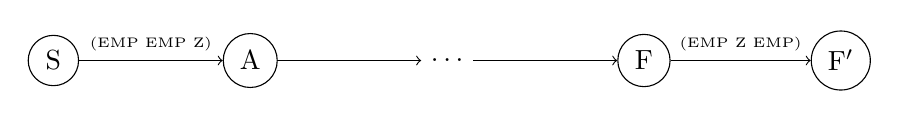
\begin{tikzpicture}
\node[circle,draw] (S) at (0,0) {S};
\node[circle,draw] (A) at (2.5,0) {A};
\node (D) at (5,0) {\dotss};
\node[circle,draw] (F) at (7.5,0) {F};
\node[circle,draw] (FF) at (10,0) {F$^{\prime{}}$};
\draw[->] (S) -- (A) node[midway,above] {\tiny{(EMP EMP Z)}};
\draw[->] (A) -- (D);
\draw[->] (D) -- (F);
\draw[->] (F) -- (FF) node[midway,above] {\tiny{(EMP Z EMP)}};
\end{tikzpicture}
\end{center}

\item<2-> The middle part simulates the given \pda{}

\item<2-> The grammar that is constructed shall simulate the simple \pda{}

\item<2-> Generate all words that take the simple \pda{} from \texttt{A} to \texttt{F$^{\prime{}}$} by popping \texttt{Z}

\item<3-> We may represent these words as a triple: \texttt{(S Z F$^{\prime{}}$)}

\item<3-> This means that the starting nonterminal for the constructed grammar, \texttt{S}, must generate \texttt{(S Z F$^{\prime{}}$)}:
\begin{alltt}
     S \arrow (A Z F\(\sp{\prime{}}\))
\end{alltt}

\end{itemize}
\end{tiny}
\end{frame}

\begin{frame}[fragile]
\frametitle{Equivalence of \pda{}s and \cfg{}s}
%\framesubtitle{HOMEWORK}
\begin{tiny}
\begin{itemize}
\item<1-> Triples need to be converted to symbols

\item<1-> We shall talk about all words that take the simple \pda{} from some state \texttt{Q} to some state \texttt{R} by popping $\theta$: \texttt{(Q $\theta$ R)}

\item<1-> All such triples represent the nonterminals of the grammar that is constructed and are formally defined as follows:
\begin{alltt}
  ;; An list nonterminal, lnt, is a (list state symbol state).

  ;; Interpretation:
  ;;   All words that take the pda from the first state to
  ;;   the second state by popping the symbol off the stack.
\end{alltt}

\item<2-> We define a \cfg{}-rule's left-hand side as follows:
\begin{alltt}
  ;; A lhs is either:
  ;;  1. symbol
  ;;  2. lnt

  ;; Interpretation:
  ;;  The left-hand side of a cfg-rule is represented as either a
  ;;  a symbol or an lnt.
\end{alltt}

\item<3-> How can the right-hand side of a \cfg{}-rule be represented?

\item<3-> Simple \pda{} rules vary in what is pushed

\item<3-> Rules that push 0 elements: \texttt{((Q a $\beta$) (R EMP))}

\item<3-> After using this rule the machine may transition in zero or more steps to an arbitrary state \texttt{V}:
\begin{center}
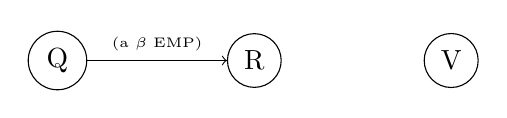
\begin{tikzpicture}
\node[circle,draw] (Q) at (0,0) {Q};
\node[circle,draw] (R) at (2.5,0) {R};
\node[circle,draw] (V) at (5,0) {V};
\draw[->] (Q) -- (R) node[midway,above] {\tiny{(a $\beta$ EMP)}};
\end{tikzpicture}
\end{center}

\item<4-> The grammar needs to generate all words that take the simple \pda{} from \texttt{Q} to \texttt{V} by popping \texttt{$\beta$} and pushing nothing

\item<4-> Such words are generated by \texttt{(Q $\beta$ V)}

\item<4-> To get to \texttt{V}, the machine reads \texttt{a} to reach \texttt{R} and then pops nothing to reach \texttt{V} in zero or more moves

\item<5-> The needed rule is:
\begin{alltt}
     (Q \(\beta\) V) \arrow a(R EMP V)
\end{alltt}

\item<5-> The right-hand side of a \cfg{}-rule may be represented by a symbol followed by an \texttt{lnt}.

\end{itemize}
\end{tiny}
\end{frame}

\begin{frame}[fragile]
\frametitle{Equivalence of \pda{}s and \cfg{}s}
%\framesubtitle{HOMEWORK}
\begin{tiny}
\begin{itemize}
\item<1-> Consider the \cfg{}-rule needed when a single element is pushed:
\begin{center}
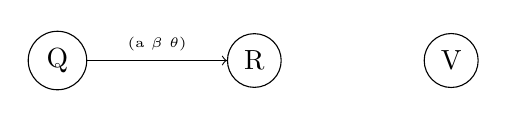
\begin{tikzpicture}
\node[circle,draw] (Q) at (0,0) {Q};
\node[circle,draw] (R) at (2.5,0) {R};
\node[circle,draw] (V) at (5,0) {V};
\draw[->] (Q) -- (R) node[midway,above] {\tiny{(a $\beta$ $\theta$)}};
\end{tikzpicture}
\end{center}

\item<2-> The grammar needs to generate all words that take the simple \pda{} from \texttt{Q} to \texttt{V} by popping \texttt{$\beta$} and pushing \texttt{$\theta$}

\item<2-> Similar to pushing nothing except that after reaching \texttt{R} \texttt{$\theta$} must be popped

\item<2-> The needed \cfg{}-rule is:
\begin{alltt}
     (Q \(\beta\) V) \arrow a(R \(\theta\) V)
\end{alltt}

\end{itemize}
\end{tiny}
\end{frame}

\begin{frame}[fragile]
\frametitle{Equivalence of \pda{}s and \cfg{}s}
%\framesubtitle{HOMEWORK}
\begin{scriptsize}
\begin{itemize}
\item<1-> Consider the \pda-rules that push two elements: \texttt{((Q a $\beta$) (R $\theta\tau$))}.
\item<1-> After popping the first element the machine may be in an arbitrary state \texttt{W}. Graphically, consider the following:
\begin{center}
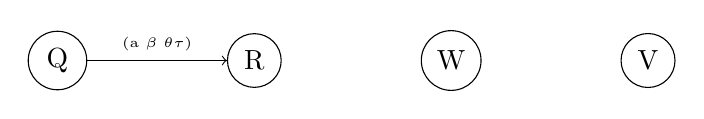
\begin{tikzpicture}
\node[circle,draw] (Q) at (0,0) {Q};
\node[circle,draw] (R) at (2.5,0) {R};
\node[circle,draw] (V) at (5,0) {W};
\node[circle,draw] (V) at (7.5,0) {V};
\draw[->] (Q) -- (R) node[midway,above] {\tiny{(a $\beta$ $\theta\tau$)}};
\end{tikzpicture}
\end{center}

\item<2-> The grammar must be able to generate a word that starts with \texttt{a} followed by a word that takes the simple \pda{} from \texttt{R} to \texttt{W} by popping $\theta$ and ending with a word that takes it from \texttt{W} to \texttt{V} by popping $\tau$

\item<2-> The needed \cfg{}-rule may be represented as follows:
\begin{alltt}
     (Q \(\beta\) V) \arrow a(R \(\theta\) W)(W \(\tau\) V)
\end{alltt}

\end{itemize}
\end{scriptsize}
\end{frame}

\begin{frame}[fragile]
\frametitle{Equivalence of \pda{}s and \cfg{}s}
%\framesubtitle{HOMEWORK}
\begin{scriptsize}
\begin{itemize}
\item<1-> Finally, we must consider the stopping conditions for word generation by the grammar

\item<1-> The three types of production rules generated above always generate at least one \texttt{lnt}

\item<2-> Once all the terminal symbols are generated, remaining nonterminals must be eliminated

\item<2-> If simple \pda{} is in an arbitrary state \texttt{Q} then it may remain in \texttt{Q} without popping or consuming any input:
\begin{alltt}
     \(\forall\)Q\(\in\)(sm-states P\(\sp{\prime{}}\)) (Q EMP Q) \arrow EMP
\end{alltt}

\item<3-> The representation of the right-hand side of a \cfg{}-rule has variety and may be defined as follows:
\begin{alltt}
  ;; A rhs is either:
  ;;  1. symbol
  ;;  2. (list symbol lnt)
  ;;  3. (list symbol lnt lnt)
  ;; Interpretation:
  ;;  A cfg-rule right hand side is represented as either a
  ;;  symbol or a list with a symbol and either one or two lnt.
\end{alltt}

\item<3-> We can now define the representation of a \cfg{}-rule as follows:
\begin{alltt}
  ;; A cfg-rl is a (list lhs ARROW rhs)
  ;; Interpretation:
  ;;   A cfg-rl represents a cfg-fule as a list with an lhs,
  ;;   an ARROW, and a rhs.
\end{alltt}

\item<4-> \textcolor{darkgreen}{Implementation in the textbook}

\end{itemize}
\end{scriptsize}
\end{frame}

\begin{frame}[fragile]
\frametitle{Equivalence of \pda{}s and \cfg{}s}
%\framesubtitle{HOMEWORK}
\begin{scriptsize}
\begin{itemize}
\item<1-> HOMEWORK: 7

\end{itemize}
\end{scriptsize}
\end{frame}


\section{Properties of CFLs}

\begin{frame}[fragile]
\frametitle{Properties of CFLs}
%\framesubtitle{HOMEWORK}
\begin{scriptsize}
\begin{itemize}
\item<1-> For every context-free \texttt{L} there is a \cfg{} that generates its members and a \pda{} that accepts its members

\item<1-> We e shall study closure properties of context-free languages and how to prove that a language is not context-free

\end{itemize}
\end{scriptsize}
\end{frame}

\begin{frame}[fragile]
\frametitle{Properties of CFLs}
%\framesubtitle{HOMEWORK}
\begin{tiny}
\begin{itemize}
\item<1-> Context-free languages are closed under union

\item<2-> Design Idea

\item<3-> If \texttt{\texttt{L$_{\texttt{1}}$}} and \texttt{\texttt{L$_{\texttt{2}}$}} are context-free languages then there are \cfg{}s, \texttt{G$_1$} and \texttt{G$_2$}, such that \texttt{\texttt{L$_{\texttt{1}}$} = L(G$_1$)} and \texttt{\texttt{L$_{\texttt{2}}$} = L(G$_2$)}

\item<3-> Without loss of generality, we assume that \texttt{(grammar-nts G$_1$) $\cap$ (grammar-nts G$_2$) = $\varnothing$}

\item<4-> The grammar for \texttt{\texttt{L$_{\texttt{1}}$} $\cup$ \texttt{L$_{\texttt{2}}$}} nondeterministically decides to simulate a derivation using \texttt{G$_1$} or \texttt{G$_2$}.


\item<5-> A \cfg{} for \texttt{\texttt{L$_{\texttt{1}}$} $\cup$ \texttt{L$_{\texttt{2}}$}} is built using the following components:
\begin{quote}
\begin{tabular}{lcl}
  %\hline
  % after \\: \hline or \cline{col1-col2} \cline{col3-col4} ...
  V    & = & \texttt{(grammar-nts G$_1$) $\cup$ (grammar-nts G$_2$) $\cup$ \{A\}}\\ %\hline
  \sig & = & \texttt{(grammar-sigma G$_1$) $\cup$ (grammar-sigma G$_2$)} \\ %\hline
  R    & = & \texttt{(grammar-rules G$_1$) $\cup$ (grammar-rules G$_2$) $\cup$} \\
       &   & \texttt{\{(S ARROW (grammar-start G$_1$)) (S ARROW (grammar-start G$_2$))\}}  \\ %\hline
  S    & = & \texttt{A = (generate-symbol \quot{}S (append (grammar-nts G$_1$) (grammar-nts G$_2$)))} \\ %\hline
\end{tabular}
\end{quote}

\end{itemize}
\end{tiny}
\end{frame}

\begin{frame}[fragile]
\frametitle{Properties of CFLs}
%\framesubtitle{HOMEWORK}
\begin{tiny}
\begin{itemize}
\item<1->
\begin{alltt}
;; cfg cfg \arrow cfg
;; Purpose: Construct a grammar for the union of the given grammars
(define (cfg-union G1 G2 #:rejects [rejs \quot{}()] #:accepts [accs \quot{}()])
\end{alltt}

\item<3->
\begin{alltt}
  (let* [(H (grammar-rename-nts (grammar-nts G1) G2))
\end{alltt}

\item<4->
\begin{alltt}
         (G-nts (grammar-nts G1))     (H-nts (grammar-nts H))
         (G-sigma (grammar-sigma G1)) (H-sigma (grammar-sigma H))
         (G-rules (grammar-rules G1)) (H-rules (grammar-rules H))
         (G-start (grammar-start G1)) (H-start (grammar-start H))
\end{alltt}

\item<5->
\begin{alltt}
         (A (gen-nt (append G-nts H-nts)))]
\end{alltt}

\item<6->
\begin{alltt}
    (make-cfg (cons A (append G-nts H-nts))
              (remove-duplicates (append G-sigma H-sigma))
              (append (list (list A ARROW G-start)
                            (list A ARROW H-start))
                      G-rules
                      H-rules)
              A
              #:rejects rejs
              #:accepts accs)))
\end{alltt}

\item<2->
\begin{alltt}
(define a2nb2nUnumb>numa (cfg-union a2nb2n
                                    numb>numa
                                    #:rejects \quot{}((b a) (b a a a b b))
                                    #:accepts \quot{}((a b) (a a b b) (b b) (b a a b b))))
(define numb>numaUMULT3-as (cfg-union numb>numa
                                      MULT3-as
                                      #:rejects \quot{}((a a a a b b) (a a))
                                      #:accepts \quot{}((b b b) (a b a b a b))))

\end{alltt}

\end{itemize}
\end{tiny}
\end{frame}

\begin{frame}[fragile]
\frametitle{Properties of CFLs}
%\framesubtitle{HOMEWORK}
\begin{scriptsize}
\begin{theorem}
\label{union-cfl-thm}
Context-free languages are closed under union.
\end{theorem}

\begin{itemize}

\item<1-> Assume S \arrow$_{G}$ w

\item<2-> By construction of \texttt{G}, the derivation of \texttt{w} starts with \texttt{(grammar-start G)} and then either \texttt{(grammar-start G1)} is generated or \texttt{(grammar-start G2)} is generated

\item<3-> If \texttt{(grammar-start G1)} is generated then \texttt{G} simulates \texttt{G1}

\item<3-> If \texttt{(grammar-start G2)} is generated then \texttt{G} simulates \texttt{G2}

\item<4-> Recall that \texttt{(grammar-nts G1)}$\cap$\texttt{(grammar-nts G2)} = $\varnothing$

\item<4-> This means that either \texttt{G1} generates \texttt{w} or \texttt{G2} generates \texttt{w}

\item<4-> Thus, \texttt{w $\in$ L(G1)$\cup$L(G2)}.

\end{itemize}
\end{scriptsize}
\end{frame}

\begin{frame}[fragile]
\frametitle{Properties of CFLs}
%\framesubtitle{HOMEWORK}
\begin{scriptsize}
\begin{itemize}
\item<1-> HOMEWORK: 1

\end{itemize}
\end{scriptsize}
\end{frame}

\begin{frame}[fragile]
\frametitle{Properties of CFLs}
%\framesubtitle{HOMEWORK}
\begin{scriptsize}
\begin{itemize}
\item<1-> Context-free languages are closed under concatenation.

\item<2-> Design Idea

\item<2-> There are \cfg{}s, \texttt{G$_{\texttt{1}}$} and \texttt{G$_{\texttt{2}}$}, such that \texttt{L$_{\texttt{1}}$ = L(\texttt{G$_{\texttt{1}}$})} and \texttt{L$_{\texttt{2}}$ = L(\texttt{G$_{\texttt{2}}$})}

\item<3-> Without loss of generality, we assume that \texttt{(grammar-nts G$_{\texttt{1}}$) $\cap$ (grammar-nts G$_{\texttt{2}}$) = $\varnothing$}

\item<3-> We shall build a grammar, \texttt{G}, for \texttt{L$_{\texttt{1}}$}\texttt{L$_{\texttt{2}}$}.


\item<4-> Every word in \texttt{L$_{\texttt{1}}$}\texttt{L$_{\texttt{2}}$} may be written as \texttt{w = xy}, such that \texttt{x} $\in$ \texttt{L$_{\texttt{1}}$} and \texttt{y} $\in$ \texttt{L$_{\texttt{2}}$}

\item<5-> A \cfg{} for \texttt{L$_{\texttt{1}}$}\texttt{L$_{\texttt{2}}$} is built using the following components:
%\begin{quote}
\begin{tabular}{lcl}
  %\hline
  % after \\: \hline or \cline{col1-col2} \cline{col3-col4} ...
  V    & = & \texttt{(grammar-nts G$_{\texttt{1}}$) $\cup$ (grammar-nts G$_{\texttt{2}}$) $\cup$ \{A\}}\\ %\hline
  \sig & = & \texttt{(grammar-sigma G$_{\texttt{1}}$) $\cup$ (grammar-sigma G$_{\texttt{2}}$)} \\ %\hline
  R    & = & \texttt{(grammar-rules G$_{\texttt{1}}$) $\cup$ (grammar-rules G$_{\texttt{2}}$) $\cup$} \\
       &   & \texttt{\{S ARROW (grammar-start G$_{\texttt{1}}$)(grammar-start G$_{\texttt{2}}$)\}}  \\ %\hline
  S    & = & \texttt{A = (generate-symbol \quot{}S (append (grammar-nts G$_1$) (grammar-nts G$_2$)))} \\ %\hline
\end{tabular}
%\end{quote}

\end{itemize}
\end{scriptsize}
\end{frame}

\begin{frame}[fragile]
\frametitle{Properties of CFLs}
%\framesubtitle{HOMEWORK}
\begin{tiny}
\begin{itemize}
\item<1->
\begin{alltt}
;; cfg cfg \arrow cfg
;; Purpose: Build a cfg for the concatenation of the \textmd{given} cfgs
(define (cfg-concat G1 G2 #:rejects [rejs \quot{}()] #:accepts [accs \quot{}()])
\end{alltt}

\item<3->
\begin{alltt}
  (let* [(G2 (grammar-rename-nts (grammar-nts G1) G2))
\end{alltt}

\item<4->
\begin{alltt}
         (G1-nts   (grammar-nts G1))   (G2-nts (grammar-nts G2))
         (G1-sigma (grammar-sigma G1)) (G2-sigma (grammar-sigma G2))
         (G1-rules (grammar-rules G1)) (G2-rules (grammar-rules G2))
         (G1-start (grammar-start G1)) (G2-start (grammar-start G2))
\end{alltt}

\item<5->
\begin{alltt}
         (A (gen-nt (append G1-nts G2-nts)))]
\end{alltt}

\item<6->
\begin{alltt}
    (make-cfg (cons A (append G1-nts G2-nts))
              (remove-duplicates (append G1-sigma G2-sigma))
              (append
                (list (list A ARROW (los->symbol (list G1-start G2-start))))
                G1-rules
                G2-rules)
              A
              #:rejects rejs
              #:accepts accs)))
\end{alltt}

\item<2->
\begin{alltt}
;; Tests for cfg-concat
(define a2nb2n-numb>numa (cfg-concat a2nb2n
                                     numb>numa
                                     #:rejects \quot{}((b a) (a a a) (a a b b))
                                     #:accepts \quot{}((b b b) (a b b) (a a b b b b b))))
(define MULT3-as-a2nb2n (cfg-concat MULT3-as
                                    a2nb2n
                                    #:rejects \quot{}((a a) (b b b b a))
                                    #:accepts \quot{}((a a b b) (b b b b b b))))

\end{alltt}

\end{itemize}
\end{tiny}
\end{frame}

\begin{frame}[fragile]
\frametitle{Properties of CFLs}
%\framesubtitle{HOMEWORK}
\begin{scriptsize}
\begin{theorem}
\label{concat-cfl-thm}
Context-free languages are closed under concatenation.
\end{theorem}

\begin{itemize}
\item<1-> HOMEWORK: 2 (proof), 3

\end{itemize}
\end{scriptsize}
\end{frame}

\begin{frame}[fragile]
\frametitle{Properties of CFLs}
%\framesubtitle{HOMEWORK}
\begin{scriptsize}
\begin{itemize}
\item<1-> Context-free languages are closed under Kleene star

\item<2-> Design idea

\item<2-> Given that \texttt{L} is a context-free language, there exists a \texttt{G} = \texttt{(make-cfg N \sig{} R S)} such that \texttt{L} = \texttt{L(G)}

\item<3-> A \cfg{} for \texttt{L$^{\texttt{*}}$} must generate 0 or more words in \texttt{L}

\item<4-> Each word in \texttt{L} is generated by \texttt{S}

\item<4-> A \cfg{} for \texttt{L$^{\texttt{*}}$} must generate 0 or more \texttt{S}s.

\item<5-> A \cfg{} for \texttt{L$^{\texttt{*}}$} may be constructed using the following components:
\begin{quote}
\begin{tabular}{lcl}
  %\hline
  % after \\: \hline or \cline{col1-col2} \cline{col3-col4} ...
  V    & = & \texttt{(grammar-nts G) $\cup$ \{A\}}\\ %\hline
  \sig & = & \texttt{(grammar-sigma G)} \\ %\hline
  R    & = & \texttt{(grammar-rules G) $\cup$ \{(S ARROW EMP) (S ARROW SS\} } \\ %\hline
  S    & = & \texttt{A = (generate-symbol \quot{}S (grammar-nts G))} \\ %\hline
\end{tabular}
\end{quote}

\end{itemize}
\end{scriptsize}
\end{frame}

\begin{frame}[fragile]
\frametitle{Properties of CFLs}
%\framesubtitle{HOMEWORK}
\begin{scriptsize}
\begin{itemize}
\item<1-> QUIZ: 4-5 (due in a week)

\end{itemize}
\end{scriptsize}
\end{frame}

\begin{frame}[fragile]
\frametitle{Properties of CFLs}
%\framesubtitle{HOMEWORK}
\begin{scriptsize}
\begin{itemize}
\item<1-> Like regular languages, context-free languages are infinite and exhibit periodicity

\item<2-> There are languages that are not context-free

\item<2-> We shall prove a pumping theorem for context-free languages

\end{itemize}
\end{scriptsize}
\end{frame}

\begin{frame}[fragile]
\frametitle{Properties of CFLs}
%\framesubtitle{HOMEWORK}
\begin{scriptsize}
\begin{itemize}
\item<1-> To simplify our work, bound a parse tree's yield length

\item<2-> Define $\kappa$ as the longest righthand side of any rule:
\begin{alltt}
;; L = a^nb^n
(define a2nb2n (make-cfg \quot{}(S)
                         \quot{}(a b)
                         \qquot{}((S ,ARROW ,EMP)
                           (S ,ARROW aSb))
                         \quot{}S))

;; L = {w | w in (a b)* AND  w has more b than a}
(define numb>numa (make-cfg \quot{}(S A)
                            \quot{}(a b)
                            \qquot{}((S ,ARROW b)
                              (S ,ARROW AbA)
                              (A ,ARROW AaAbA)
                              (A ,ARROW AbAaA)
                              (A ,ARROW ,EMP)
                              (A ,ARROW bA))
                            \quot{}S))
\end{alltt}

\item<2-> For \texttt{a2nb2n}, $\kappa$ is 3 because its longest righthand side is \texttt{aSb}

\item<2-> For \texttt{numb>numa}, $\kappa$ is 5.

\item<3-> Given a \cfg{} \texttt{G}, the yield's length for any parse tree is bounded by the height of the tree and $\kappa$

\end{itemize}
\end{scriptsize}
\end{frame}

\begin{frame}[fragile]
\frametitle{Properties of CFLs}
%\framesubtitle{HOMEWORK}
\begin{scriptsize}
\begin{lemma}
T's yield's length $\leq$ $\kappa^h$.
\end{lemma}

\begin{itemize}
\item<1-> The proof is by induction on h

\item<2-> Base case: h = 1

\item<2-> A parse tree of height 1 means that a single rule has been used

\item<2-> The yield's length $\leq$ $\kappa$ = $\kappa^1$ = $\kappa^h$

\item<3-> Inductive Step
\item<3-> Assume: T's yield's length $\leq$ $\kappa^n$, for h = n
\item<3-> Show: T's yield's length $\leq$ $\kappa^{n+1}$, for h = n + 1

\item<4-> Consider the structure of a parse tree of height n + 1
  \begin{itemize}
    \item Root
    \item At most $\kappa$ subtrees of height n
  \end{itemize}

\item<5-> Let $T_i$ be any of these subtrees

\item<5-> By inductive hypothesis, $T_i$'s yield's length $\leq \kappa^n$

\item<5-> If every $T_i$'s yield's length is $\kappa^n$ then T's yield's length is at most $\kappa * \kappa^n$


\item<5-> Thus, T's yield's length $\leq$ $\kappa^{n+1}$. $\qed$

\item<6-> Let \texttt{w$\in$L(G)} such that $|$\texttt{w}$| > \kappa^h$

\item<6-> \texttt{w}'s parse tree must have a path longer than \texttt{h}

\end{itemize}
\end{scriptsize}
\end{frame}

\begin{frame}[fragile]
\frametitle{Properties of CFLs}
%\framesubtitle{HOMEWORK}
\begin{tiny}
\begin{theorem}
If w$\in$ L(G) $\wedge$ $|$w$|$ $>$ $\kappa^{|V|}$ then w = uvxyz such that (v $\neq$ \texttt{EMP} $\vee$ y $\neq$ \texttt{EMP}), $\exists$k $|$vxy$|$ $\leq$ k, and $\forall$n$\geq$0 uv$^n$xy$^n$z $\in$ L(G).
\end{theorem}

\begin{itemize}
\item<1-> Proof

\item<2-> Let T be the parse tree for w rooted at S with the smallest number of leaves

\item<3-> $|$w$| > \kappa^{|V|} \Rightarrow$ path in T of length at least $|$V$|$ + 1

\item<3-> $|$V$|$ + 2 nodes of which the last must be a terminal symbol

\item<3-> $|$V$|$ + 1 nonterminals

\item<3-> Must have a repeated nonterminal

\item<4->
\begin{center}
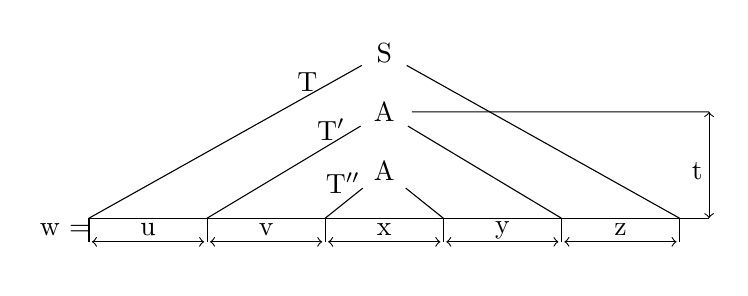
\begin{tikzpicture}[scale=0.75]
\node[circle] (T) at (3.7,2.5) {T};
\node[circle] (T1) at (4.1,1.7) {T$^{\prime}$};
\node[circle] (T2) at (4.3,0.8) {T$^{\prime\prime}$};
\node[circle] (T) at (10.3,1) {t};
\node[circle] (W) at (-0.4,0) {w =};
\node[circle] (U) at (1,0) {u};
\node[circle] (V) at (3,0) {v};
\node[circle] (X) at (5,0) {x};
\node[circle] (Y) at (7,0) {y};
\node[circle] (Z) at (9,0) {z};
\draw[] (0,0.2) -- (10.5,0.2); % line above letters
\draw[] (0,0.2) -- (0,-0.2); % bars between letters
\draw[] (2,0.2) -- (2,-0.2);
\draw[] (4,0.2) -- (4,-0.2);
\draw[] (6,0.2) -- (6,-0.2);
\draw[] (8,0.2) -- (8,-0.2);
\draw[] (10,0.2) -- (10,-0.2);
\draw[<->] (0.05,-0.2) -- (1.95,-0.2);  % double arrorws below arrows
\draw[<->] (2.05,-0.2) -- (3.95,-0.2);
\draw[<->] (4.05,-0.2) -- (5.95,-0.2);
\draw[<->] (6.05,-0.2) -- (7.95,-0.2);
\draw[<->] (8.05,-0.2) -- (9.95,-0.2);
\node[circle] (S) at (5,3) {S};
\node[circle] (A) at (5,2) {A};
\node[circle] (B) at (5,1) {A};
\draw[] (0,0.2) -- (S);
\draw[] (S) -- (10,0.2);
\draw[] (A) -- (2,0.2);
\draw[] (A) -- (8,0.2);
\draw[] (B) -- (4,0.2);
\draw[] (B) -- (6,0.2);
\draw[<->] (10.5,2) -- (10.5,0.2);  % double arrorws height of T'
\draw[] (A) -- (10.5,2);  % double arrorws height of T'
\end{tikzpicture}
\end{center}

\item<4-> Observe that the part of T$^{\prime}$ excluding T$^{\prime\prime}$ may be repeated an arbitrary number of times or may be excluded resulting in a word that is in L(G)

\item<4-> uv$^n$x$y^n$z$\in$L(G) for n$\geq$0

\item<5-> Let t be the height of T$^{\prime}$

\item<5-> The yield of T$^{\prime}$, vxy, has a length of at most $\kappa^t$

\item<5-> This is the constant k that bounds the length of the subword that contains the parts that may be repeated an arbitrary number of times: $|$vxy$| \leq \kappa^t = k$

\item<6-> Finally, observe that if vy = EMP then there is a parse tree with fewer leaves that generates w:
\begin{alltt}
     S \arrow\(\sp{*}\) uAz \arrow\(\sp{*}\) uxz = w
\end{alltt}

\item<6-> Smaller parse tree omits the derivation of A from A

\item<6-> Contradicts our assumption that T is the parse tree for w with the smallest number of leaves

\item<6-> Therefore, vy $\neq$ EMP $\Rightarrow$ $0<|vxy|\leq{}k\leq\kappa^{|V|}$ $\qed$

\end{itemize}
\end{tiny}
\end{frame}

\begin{frame}[fragile]
\frametitle{Properties of CFLs}
%\framesubtitle{HOMEWORK}
\begin{tiny}
\begin{theorem}
L = \{a$^{\texttt{n}}$b$^{\texttt{n}}$c$^{\texttt{n}} | $ n $\geq$ 0\} is not context-free.
\end{theorem}

\begin{itemize}
\item<1-> \noindent Let w = a$^k$b$^k$c$^k$

\item<2-> We must determine the possible values \texttt{vxy} may take

\item<2-> \texttt{vxy} may not contains \texttt{a}s, \texttt{b}s, and \texttt{c}s because the length of \texttt{vxy} must be less than or equal to \texttt{k}

\item<2-> \texttt{vxy} may contain only one letter variety or may contain two letter varieties by straddling the border between \texttt{a}s and \texttt{b}s or between \texttt{b}s and \texttt{c}s

\item<3-> We prove that \texttt{L} is not context-free as follows:\\
\begin{tabular}{ll}
  %\hline
  % after \\: \hline or \cline{col1-col2} \cline{col3-col4} ...
             &  \\
  \texttt{vxy}        & \textrm{Argument} \\
             & \\
  a$^+$      & Pump up once on v and y. The resulting word has more \texttt{a}s than \texttt{b}s \\
             & and than \texttt{c}s. Therefore, it is not in \texttt{L}. \\
  b$^+$      & Pump up once on v and y. The resulting word has more \texttt{b}s than \texttt{a}s \\
             & and than \texttt{c}s. Therefore, it is not in \texttt{L}. \\
  c$^+$      & Pump up once on v and y. The resulting word has more \texttt{c}s than \texttt{a}s \\
             & and than \texttt{b}s. Therefore, it is not in \texttt{L}. \\
  a$^+$b$^+$ & Pump up once on v and y. The resulting word has a \texttt{b} before an \texttt{a}. \\
             & Therefore, it is not in \texttt{L}. \\
  b$^+$c$^+$ & Pump up once on v and y. The resulting word has a \texttt{c} before a \texttt{b}. \\
             & Therefore, it is not in \texttt{L}. \\
\end{tabular}

\item<3-> No matter where the \texttt{vxy} window is placed in \texttt{w}, a word that is not in \texttt{w} may be generated

\item<3-> We may conclude that \texttt{L} is not context-free. $\qed$

\end{itemize}
\end{tiny}
\end{frame}

\begin{frame}[fragile]
\frametitle{Properties of CFLs}
%\framesubtitle{HOMEWORK}
\begin{scriptsize}
\begin{theorem}
L = \{a$^{\texttt{n}}$ $|$ n is a square\} is not context-free.
\end{theorem}

\begin{itemize}
\item<1-> Let w = a$^{k^2}$

\item<2-> \texttt{vy} = \texttt{a}$^i$, where $i > 0$

\item<3-> If we pump up once the resulting word is a$^{K^2 + i}$

\item<4-> Observe that there are no words in \texttt{L} with a length greater than $|a^{K^2}|$ and less than $|a^{(k+1)^2}|$

\item<4->  After a$^{k^2}$ the next word in \texttt{L} has length K$^2$ + 2K + 1

\item<5-> In order for a$^{k^2 + i}$ to be in \texttt{L}, i must at a minimum be of length 2k + 1

\item<5->  Impossible because $|$vxy$|$ must be less than or equal to k

\item<5-> i cannot be greater than or equal to 2k + 1

\item<6-> No matter where the \texttt{vxy} window is placed in \texttt{w}, a word that is not in \texttt{w} may be generated

\item<6-> Therefore, we may conclude that \texttt{L} is not context-free $\qed$

\end{itemize}
\end{scriptsize}
\end{frame}

\begin{frame}[fragile]
\frametitle{Properties of CFLs}
%\framesubtitle{HOMEWORK}
\begin{scriptsize}
\begin{itemize}
\item<1-> HOMEWORK: 6, 7, 9, 10

\end{itemize}
\end{scriptsize}
\end{frame}

\begin{frame}[fragile]
\frametitle{Properties of CFLs}
%\framesubtitle{HOMEWORK}
\begin{scriptsize}
\begin{theorem}
Context-free languages are not closed under intersection.
\end{theorem}

\begin{itemize}
\item<1-> Proof

\item<2-> Let L$_1$ = \{a$^n$b$^n$c$^m$ $|$ m,n $\geq$ 0\}

\item<2-> L$_2$ = \{a$^m$b$^n$c$^n$ $|$ m,n $\geq$ 0\}

\item<2-> Both are context-free

\item<3-> Consider L = L$_1$ $\cap$ L$_2$

\item<4-> L = \{a$^n$b$^n$c$^n$ $|$ n $\geq$ 0\}, which we know is not context-free

\item<4-> Therefore, context-free languages are not closed under intersection.

\end{itemize}
\end{scriptsize}
\end{frame}

\begin{frame}[fragile]
\frametitle{Properties of CFLs}
%\framesubtitle{HOMEWORK}
\begin{scriptsize}
\begin{theorem}
Context-free languages are not closed under complement.
\end{theorem}

\begin{itemize}
\item<1-> Proof

\item<2-> \texttt{L$_1$ $\cap$ L$_2$} = \texttt{(complement ((complement L$_1$) $\cup$ (complement L$_2$)))}

\item<2-> If context-free languages were closed under complement then they would also be closed under intersection, which we know they are not

\item<2-> Therefore, context free languages are not closed under complement

\end{itemize}
\end{scriptsize}
\end{frame}

\begin{frame}[fragile]
\frametitle{Properties of CFLs}
%\framesubtitle{HOMEWORK}
\begin{scriptsize}
\begin{itemize}
\item<1-> Although context-free languages are not closed under intersection, there exist context-free languages that result in a context-free language when intersected

\item<2-> Recall that all regular languages are context-free

\item<2-> The intersection of a context-free language and a regular language is a context-free language

\item<2-> How can we prove this?

\item<3-> Develop a new constructor for a context-free language: constructive proof

\end{itemize}
\end{scriptsize}
\end{frame}

\begin{frame}[fragile]
\frametitle{Properties of CFLs}
%\framesubtitle{HOMEWORK}
\begin{scriptsize}
\begin{itemize}
\item<1-> Design Idea

\item<2-> Have a \pda{}: \texttt{M$_1$ = (make-ndpda K$_1$ \sig{}$_1$ \gam{} S$_1$ F$_1$ R$_1$)}

\item<2-> Have a \dfa{}: \texttt{M$_2$ = (make-dfa K$_2$ \sig{}$_2$ S$_2$ F$_2$ R$_2$)}

\item<3-> Build a \pda{} that simultaneously simulates \texttt{M$_1$} and \texttt{M$_2$}

\item<3-> Only accept if both \texttt{M$_1$} and \texttt{M$_2$} accept.

\item<4-> Basic idea: Each state of the new \pda{} be a \emph{super state} that represents a state in \texttt{M$_1$} and a state in \texttt{M$_2$}

\item<4-> Simulate all the transitions of \texttt{M$_1$} and track the transitions made by \texttt{M$_2$}

\item<4-> If \texttt{M$_1$} has a rule that moves from \texttt{P} to \texttt{Q} on an \texttt{a} then for every state \texttt{Y}$\in$\texttt{M$_2$} the new \pda{} has a rule that moves from super state \texttt{(P Y)} to super state \texttt{(Q T)}

\item<4-> If \texttt{M$_1$} has a rule that moves from \texttt{P} to \texttt{Q} on \texttt{EMP} then for every state \texttt{Y}$\in$\texttt{M$_2$} the new \pda{} has a rule that moves from super state \texttt{(P Y)} to super state \texttt{(Q Y)} to simulate that \texttt{M$_2$} does not change state

\item<5->
\begin{alltt}
     ;; Push or pop elements, stacke, is either
     ;;  1. EMP
     ;;  2. (listof symbol)

     ;; A super state, ss, is a (list state state)

     ;; A pda super rule, ssrule, is:
     ;;  (list (list ss symbol stacke) (list ss stacke))
\end{alltt}

\end{itemize}
\end{scriptsize}
\end{frame}

\begin{frame}[fragile]
\frametitle{Properties of CFLs}
%\framesubtitle{HOMEWORK}
\begin{tiny}
\begin{itemize}
\item<1->
\begin{alltt}
;; pda dfa \arrow pda  Purpose: Build intersection pda from given machines
(define (pda-intersect-dfa a-pda a-dfa #:rejects [rejs \quot{}()] #:accepts [accs \quot{}()])
\end{alltt}

\item<7->
\begin{alltt}
  ;; (listof state) (listof state) \arrow (listof ss)
  ;; Purpose: Create a list of super states
  (define (cartesian-product pda-sts dfa-sts) \dotss)
  ;; (listof pda-rule) (listof state) \arrow (listof ssrule)
  ;; Purpose: Create ssrules for given empty transition pda-rules
  (define (make-EMP-rls EMP-pda-rls dfa-sts) \dotss)
  ;; (listof pda-rule) (listof state) (listof dfa-rls) \arrow (listof ssrule)
  ;; Purpose: Create ssrules for given nonempty transition pda-rules
  (define (make-nonEMP-rls non-EMP-pda-rls dfa-sts dfa-rls) \dotss)
  ;; (listof ss) \arrow (listof (list ss state))
  ;; Purpose: Create table associating given super states with a new state
  (define (make-ss-table K) \dotss)
  ;; (listof ssrule) (ss \arrow state) \arrow (listof pda-rule)
  ;; Purpose: Convert ssrules to pda-rules
  (define (convert-ssrules ss-rls ss->state) \dotss)
\end{alltt}

\item<2->
\begin{alltt}
 (let* [(pda-sts (sm-states a-pda))  (dfa-sts (sm-states a-dfa))
        (pda-rls (sm-rules a-pda))   (dfa-rls (sm-rules a-dfa))
\end{alltt}

\item<3->
\begin{alltt}
        (K (cartesian-product pda-sts dfa-sts))
        (start (list (sm-start a-pda) (sm-start a-dfa)))
        (F (cartesian-product (sm-finals a-pda) (sm-finals a-dfa)))
\end{alltt}

\item<4->
\begin{alltt}
        (non-EMP-pda-rls (filter (\lamb (r) (not (eq? (second (first r)) EMP))) pda-rls))
        (EMP-pda-rls (filter (\lamb (r) (eq? (second (first r)) EMP)) pda-rls))
        (non-EMP-rls (make-nonEMP-rls non-EMP-pda-rls dfa-sts dfa-rls))
        (EMP-rls (make-EMP-rls EMP-pda-rls dfa-sts))
\end{alltt}

\item<5->
\begin{alltt}
        (ss-tbl (make-ss-table K))
        (ss->state (\lamb (ss) (second (assoc ss ss-tbl))))]
\end{alltt}

\item<6->
\begin{alltt}
   (make-ndpda (map ss->state K)  (sm-sigma a-pda)  (sm-gamma a-pda)
               (ss->state start)  (map ss->state F)
               (convert-ssrules (append non-EMP-rls EMP-rls) ss->state)
               #:rejects rejs
               #:accepts accs)))
\end{alltt}

\end{itemize}
\end{tiny}
\end{frame}

\begin{frame}[fragile]
\frametitle{Properties of CFLs}
%\framesubtitle{HOMEWORK}
\begin{tiny}
\begin{itemize}
\item<1->
\begin{alltt}
     ;; (listof state) (listof state) \arrow (listof ss)
     ;; Purpose: Create a list of super states
     (define (cartesian-product pda-sts dfa-sts)
       (for*/list [(s1 pda-sts) (s2 dfa-sts)] (list s1 s2)))
\end{alltt}

\item<2->
\begin{alltt}
     (define (make-EMP-rls EMP-pda-rls dfa-sts)
       (for*/list [(r EMP-pda-rls) (s dfa-sts)]
         (list (list (list (first (first r)) s)
                     EMP
                     (third (first r)))
               (list (list (first (second r)) s)
                     (second (second r))))))
\end{alltt}

\item<3->
\begin{alltt}
     (define (make-nonEMP-rls non-EMP-pda-rls dfa-sts dfa-rls)
       (for*/list [(r non-EMP-pda-rls) (s dfa-sts)]
         (list (list
                 (list (first (first r)) s)
                 (second (first r))
                 (third (first r)))
               (list
                 (list
                   (first (second r))
                   (third
                   (first
                     (filter (\lamb (rl)
                               (and (eq? (first rl) s)
                                    (eq? (second rl)
                                         (second (first r)))))
                             dfa-rls))))
                 (second (second r))))))
\end{alltt}

\end{itemize}
\end{tiny}
\end{frame}

\begin{frame}[fragile]
\frametitle{Properties of CFLs}
%\framesubtitle{HOMEWORK}
\begin{tiny}
\begin{itemize}
\item<1->
\begin{alltt}
     (define (make-ss-table K)
       (foldl (\(\lambda\) (ss acc)
                (cons (list ss (gen-state (map second acc))) acc))
              \quot{}()
              K))

     (define (convert-ssrules ss-rls ss->state)
      (for*/list [(r ss-rls)]
       (list
        (list (ss->state (first (first r)))
              (second (first r))
              (third (first r)))
        (list (ss->state (first (second r)))
              (second (second r))))))
\end{alltt}

\item<2->
\begin{alltt}
;; Tests for pda-intersect-dfa
(define a^nb^nIM (pda-intersect-dfa a^nb^n
                                    ab*
                                    #:rejects \quot{}(() (a b b) (a a b b))
                                    #:accepts \quot{}((a b)))) \textcolor{darkgreen}{only word in the intersection}
(define a^nb^nINO-ABBA (pda-intersect-dfa a^nb^n
                                          NO-ABAA
                                          #:rejects \quot{}((b b) (a a b) (b b a a b b a b))
                                          #:accepts \quot{}(() (a a b b))))

\end{alltt}

\end{itemize}
\end{tiny}
\end{frame}

\begin{frame}[fragile]
\frametitle{Properties of CFLs}
%\framesubtitle{HOMEWORK}
\begin{scriptsize}
\begin{theorem}
\label{intersect-pda-dfa-thm}
The intersection of a context-free language and a regular language is context-free.
\end{theorem}

\begin{itemize}
\item<1-> Proof (sketch)

\item<2-> Let Q be a \pda{}, let D be a \dfa{}, and let M = (pda-intersect-dfa Q D)

\item<3-> By construction, M simulates the transitions of both Q and D

\item<3-> M starts its simulations in a state that represents Q's and D's starting states

\item<3-> Only accepts if both Q and D accept

\item<3-> This means that all accepted strings must be in L(Q) and L(D)

\item<4-> L(M) = L(Q) $\cap$ L(D). $\qed$

\end{itemize}
\end{scriptsize}
\end{frame}

\begin{frame}[fragile]
\frametitle{Properties of CFLs}
%\framesubtitle{HOMEWORK}
\begin{scriptsize}
\begin{theorem}
L = \{ w$\in$\{a b\}$^* |$ w does not contain abaa and has equal number of \texttt{a}s and \texttt{b}s.\} is context-free.
\end{theorem}

\begin{itemize}
\item<1-> The previous theorem may be used to prove a language, \texttt{L}, is context-free

\item<2-> The language of all words that do not contain abaa is decided by NO-ABAA (from dfa chapter)
\item<2-> L(NO-ABAA) is regular

\item<3-> The language, E, of all words that have an equal number of \texttt{a}s and \texttt{b}s is generated by the following context-free grammar:
\begin{alltt}
     S \arrow EMP
       \arrow aSb
       \arrow bSa
       \arrow aSbSbSa
       \arrow bSaSaSb
\end{alltt}

\item<3-> E is context-free

\item<4-> Observe that L = L(E) $\cap$ L(NO-ABAA)

\item<4-> By previous theorem, we may conclude that L is context-free. $\qed$

\end{itemize}
\end{scriptsize}
\end{frame}

\begin{frame}[fragile]
\frametitle{Properties of CFLs}
%\framesubtitle{HOMEWORK}
\begin{scriptsize}
\begin{itemize}
\item<1-> HOMEWORK: 12--14

\end{itemize}
\end{scriptsize}
\end{frame}

\section{Deterministic \pda{}s}

\begin{frame}[fragile]
\frametitle{Deterministic \pda{}s}
%\framesubtitle{HOMEWORK}
\begin{scriptsize}
\begin{itemize}
\item<1-> Now, we explore deterministic \pda{}s in more detail

\item<2-> From a given configuration, \texttt{C$_{\texttt{i}}$}, there is at most one transition that is applicable

\item<2-> The \pda{} never has a choice of what to do next

\item<3-> Such a \pda{} must satisfy the following constraints:
\begin{enumerate}
 \item There are no pair of transitions that offer a choice on which to use
 \item For all accepting states, \texttt{Q}, there are no transitions of this nature: \texttt{((Q EMP EMP) (P a))}. That is, the machine does not have to choose between continuing with the computation or accepting.
\end{enumerate}

\item<4-> Given a nondeterministic \pda{}, can a deterministic \pda{} that decides the same language be constructed?

\end{itemize}
\end{scriptsize}
\end{frame}

\begin{frame}[fragile]
\frametitle{Deterministic \pda{}s}
%\framesubtitle{HOMEWORK}
\begin{scriptsize}
\texttt{L = wcw$^{\texttt{R}}$}

\begin{itemize}
\item<1-> The nondeterministic \pda{}'s we previously designed may be summarized as follows:
\begin{enumerate}
 \item Nondeterministically move from \texttt{S}, the starting state, to \texttt{P}
 \item In \texttt{P}, accumulate \texttt{w} on the stack in reversed order and move to \texttt{Q} upon reading a \texttt{c} without modifying the stack.
 \item In \texttt{Q}, match the elements of \texttt{w$^{\texttt{R}}$} with the elements on the stack and nondeterministically move to, \texttt{F}, the final state.
\end{enumerate}

\item<2-> A deterministic \pda{} for \texttt{L} must avoid nondeterministic transitions

\item<2-> Observe that the nondeterministic \pda{} operates in two phases: before reading \texttt{c}, it pushes \texttt{w} onto the stack and after reading \texttt{c}, it matches \texttt{w$^{\texttt{R}}$} with the elements on the stack

\item<2-> The phases are clearly delineated around reading \texttt{c}

\item<3-> A deterministic \pda{} may decide \texttt{L} as follows:
\begin{enumerate}
 \item Before reading \texttt{c}, push read elements onto the stack
 \item After reading \texttt{c}, match read elements with elements onto the stack
\end{enumerate}

\end{itemize}
\end{scriptsize}
\end{frame}

\begin{frame}[fragile]
\frametitle{Deterministic \pda{}s}
%\framesubtitle{HOMEWORK}
\begin{scriptsize}
\texttt{L = wcw$^{\texttt{R}}$}

\begin{itemize}
\item<1-> Name is \texttt{dwcw\^{}r}, input alphabet is \texttt{\{a b c\}}, and the stack alphabet is \texttt{\{a b\}}.

\item<2-> Sample tests:
\begin{alltt}
(check-reject? dwcw^r \quot{}() \quot{}(a b b a) \quot{}(a a) \quot{}(a b b c b b a b))
(check-accept? dwcw^r \quot{}(a c a) \quot{}(b a c a b) \quot{}(b b a c a b b))
\end{alltt}

\end{itemize}
\end{scriptsize}
\end{frame}

\begin{frame}[fragile]
\frametitle{Deterministic \pda{}s}
%\framesubtitle{HOMEWORK}
\begin{tiny}
\texttt{L = wcw$^{\texttt{R}}$}

\begin{itemize}
\item<1->
\begin{alltt}
     S: ci = \{a b\}\(\sp{\texttt{*}}\) AND stack = ci\(\sp{\texttt{R}}\), starting state
\end{alltt}

\item<2->
\begin{alltt}
     F: ci = xycy\(\sp{\texttt{R}}\) AND stack = x\(\sp{\texttt{R}}\), final state
\end{alltt}

\item<3->
\begin{alltt}
     ((S a ,EMP) (S (a)))     ((S b ,EMP) (S (b)))     ((S c ,EMP) (F ,EMP))
\end{alltt}

\item<4->
\begin{alltt}
     ((F a (a)) (F ,EMP))     ((F b (b)) (F ,EMP))
\end{alltt}

\item<4-> There are no nondeterministic choices that the machine must make

\item<5->
\begin{alltt}
;; L = wcw^R
;; State Documentation
;;  S: ci = {a b}* AND stack = ci^R
;;  F: ci = xycy^R AND stack = x^R
(define dwcw^r (make-ndpda \quot{}(S F)
                           \quot{}(a b c)
                           \quot{}(a b)
                           \quot{}S
                           \quot{}(F)
                           \qquot{}(((S a ,EMP) (S (a)))
                             ((S b ,EMP) (S (b)))
                             ((S c ,EMP) (F ,EMP))
                             ((F a (a)) (F ,EMP))
                             ((F b (b)) (F ,EMP)))))

(check-reject? dwcw^r \quot{}() \quot{}(a b b a) \quot{}(a a) \quot{}(a b b c b b a b))
(check-accept? dwcw^r \quot{}(a c a) \quot{}(b a c a b) \quot{}(b b a c a b b))
\end{alltt}

\end{itemize}
\end{tiny}
\end{frame}

\begin{frame}[fragile]
\frametitle{Deterministic \pda{}s}
%\framesubtitle{HOMEWORK}
\begin{tiny}
\texttt{L = wcw$^{\texttt{R}}$}

\begin{itemize}
\item<1->
\begin{alltt}
     ;; word stack \arrow{} Boolean
     (define (S-INV ci s)
       (and (andmap (\lamb{} (s) (or (eq? s \quot{}a) (eq? s \quot{}b))) ci)
            (equal? ci (reverse s))))

     (check-equal? (S-INV \quot{}(c) \elist{}) #f)
     (check-equal? (S-INV \quot{}(b a) \quot{}(b a)) #f)
     (check-equal? (S-INV \elist{} \elist{}) #t)
     (check-equal? (S-INV \quot{}(a b b) \quot{}(b b a)) #t)
\end{alltt}

\item<2->
\begin{alltt}
     ;; word stack \arrow{} Boolean
     (define (F-INV ci s)
       (and (member \quot{}c ci)
            (let* [(w (takef ci (\lamb{} (x) (not (eq? x \quot{}c)))))
                   (x (take ci (length s)))
                   (y\^{}R (drop ci (add1 (length w))))]
              (and (equal?
                     ci
                     (append x (reverse y^R) (list \quot{}c) y\^{}R))
                   (equal? s (reverse x))))))

     (check-equal? (F-INV \quot{}(a b c) \elist) #f)
     (check-equal? (F-INV \quot{}(a a c) \quot{}(a)) #f)
     (check-equal? (F-INV \quot{}(a b) \quot{}(b a)) #f)
     (check-equal? (F-INV \quot{}(c) \elist) #t)
     (check-equal? (F-INV \quot{}(b a c) \quot{}(a b)) #t)
     (check-equal? (F-INV \quot{}(a b b c b) \quot{}(b a)) #t)
\end{alltt}

\end{itemize}
\end{tiny}
\end{frame}


\begin{frame}[fragile]
\frametitle{Deterministic \pda{}s}
%\framesubtitle{HOMEWORK}
\begin{tiny}
\begin{alltt}
     L = wcw\(\sp{\texttt{R}}\)        M = dwcw\string^r           v \(\in\) (sm-sigma M)\(\sp{*}\)
     s = the stack   ci = consumed input
\end{alltt}

\begin{theorem}
\label{dwcwrev-thm-inv}
The state invariants hold when M accepts v.
\end{theorem}

\begin{itemize}
\item<1-> For the base case, when \texttt{M} starts ci = \elist{} and s = \elist{}. This means that ci only contains \texttt{a}s and \texttt{b}s and that ci equals s reversed. Thus, S-INV holds.

\item<2-> Proof invariants hold after each transition that consumes input:

\item<2-> \underline{\texttt{((S a ,EMP) (S (a)))}}: By inductive hypothesis S-INV holds. This means that ci$\in$\{a b\}$^*$ and that ci = s$^R$. After using this rule, the consumed input only contains \texttt{a}s and \texttt{b}s and the consumed input is equal to the stack reversed. Thus, S-INV holds.

\item<3-> \underline{\texttt{((S b ,EMP) (S (b)))}}: By inductive hypothesis S-INV holds. This means that ci$\in$\{a b\}$^*$ and that ci = s$^R$. After using this rule, the consumed input only contains \texttt{a}s and \texttt{b}s and the consumed input is equal to the stack reversed. Thus, S-INV holds.

\item<4-> \underline{\texttt{((S c ,EMP) (F ,EMP))}}: By inductive hypothesis S-INV holds. This means that ci$\in$\{a b\}$^*$ and that ci = s$^R$. After using this rule, ci=xycy$^R$, where x$\in$\{a b\}$^*$ and y=\elist{}, and stack=x$^R$. Thus, F-INV holds. \\

\item<5-> \underline{\texttt{((F a (a)) (F ,EMP))}}: By inductive hypothesis F-INV holds. This means that ci=xycy$^R$, where x,y$\in$\{a b\}$^*$, and stack=x$^R$. Using this rule means that x's last element is an \texttt{a}. That is, x=x\quot{}a. After using this rule, ci=x\quot{}aycy$^R$a=x\quot{}ayc(ay)$^R$ and stack=x\quot{}$^R$. Thus, F-INV holds.

\item<6-> \underline{\texttt{((F b (b)) (F ,EMP))}}: By inductive hypothesis F-INV holds. This means that ci=xycy$^R$, where x,y$\in$\{a b\}$^*$, and stack=x$^R$. Using this rule means that x's last element is a \texttt{b}. That is, x=x\quot{}b. After using this rule, ci=x\quot{}bycy$^R$b=\\
\noindent x\quot{}byc(by)$^R$ and stack=x\quot{}$^R$. Thus, F-INV holds

\end{itemize}
\end{tiny}
\end{frame}


\begin{frame}[fragile]
\frametitle{Deterministic \pda{}s}
%\framesubtitle{HOMEWORK}
\begin{tiny}
\texttt{L = wcw$^{\texttt{R}}$}

\begin{itemize}
\item<1->
\begin{lemma}
\label{in-dwcwrev}
     w\(\in\)L \(\Leftrightarrow\) w\(\in\)L(M)
\end{lemma}

\item<2->
\begin{proof}
\mbox{}\\
\noindent ($\Rightarrow$) Assume w\(\in\)L. This means that w = vcv$^R$. Given that state invariants always hold, there is a computation that has M consume w and reach F with an empty stack. Therefore, w\(\in\)L(M). \\

\noindent ($\Leftarrow$) Assume w\(\in\)L(M). This means that M halts in F, the only final state, with an empty stack having consumed w. Given that the state invariants always hold we may conclude that w = vcv$^R$. Therefore, w\(\in\)L. $\qed$
\end{proof}

\item<3->
\begin{lemma}
\label{notin-dwcwrev}
     w\(\notin\)L \(\Leftrightarrow\) w\(\notin\)L(M)
\end{lemma}

\item<4->
\begin{proof}
\mbox{}\\
\noindent ($\Rightarrow$) Assume w\(\notin\)L. This means w $\neq$ v$^R$cv. Given that the state invariant predicates always hold, there is no computation that has M consume w and end in F with an empty stack. Therefore, w\(\notin\)L(M).\\

\noindent ($\Leftarrow$) Assume w\(\notin\)L(M). This means that M does not halt in F with an empty stack having consumed w. Given that the state invariants always hold, this means that w $\neq$ vcv$^R$. Thus, w\(\notin\)L. $\qed$
\end{proof}

\end{itemize}
\end{tiny}
\end{frame}

\begin{frame}[fragile]
\frametitle{Deterministic \pda{}s}
%\framesubtitle{HOMEWORK}
\begin{tiny}
\texttt{L = \{a$^{\texttt{m}}$b$^{\texttt{n}}$c$^{\texttt{p}} |$ m$\neq$n $\wedge$ m,n,p$>$0\}}

\begin{itemize}
\item<1-> Intuitively: push all the \texttt{a}s onto the stack, match \texttt{b}s, either pop excess \texttt{a}s or read excess \texttt{b}s, and read \texttt{c}s

\item<1-> Challenge: deterministically determine if excess \texttt{a}s need to be popped or excess \texttt{b}s need to be read

\item<2-> If there is an excess of \texttt{b}s in the input word then all the \texttt{a}s on the stack will be matched and the stack becomes empty

\item<2-> This is a problem because the machine cannot nondeterministically decide to keep matching \texttt{a}s on the stack or read excess \texttt{b}s

\item<3-> If the machine could sense that the stack is empty then the decision becomes deterministic

\item<3-> If the stack is empty read excess \texttt{b}s

\item<3-> Otherwise, match \texttt{a}s as \texttt{b}s are read

\item<4-> Another potential problem is deterministically transitioning to the final state

\item<4-> To prevent nondeterministic transitions of this nature, a special end of input symbol, \texttt{z}, not in the input alphabet of the machine, shall be used

\item<4-> All input: \texttt{wz}

\item<5-> How can the machine sense that the stack is empty?

\item<6-> Use a technique developed to construct simple \pda{}s: the machine shall use a bottom of the stack symbol

\item<6-> For our purposes, \texttt{y} serves as the bottom of the stack symbol.

\item<7-> The machine's phases may be outlined as follows:
\begin{enumerate}
 \item \tiny{When} started, if an \texttt{a} is read then \texttt{(a y)} is pushed onto the stack.
 \item \tiny{All} the remaining \texttt{a}s read are pushed onto the stack.
 \item \tiny{Match} a read \texttt{b} by popping an \texttt{a}
 \item \tiny{Decide} if there are more \texttt{a}s or more \texttt{b}s:
  \begin{enumerate}
    \item \tiny{If} a \texttt{c} is read and there is an \texttt{a} on the stack then there are more \texttt{a}s than \texttt{b}s. The machine transitions to a state to read the remaining \texttt{c}s and pop the remaining \texttt{a}s. Upon reading \texttt{z}, the machine pops \texttt{y} and moves to the final state.
    \item \tiny{If} a \texttt{b} is read and \texttt{y} is at the top of the stack then there are more\texttt{b}s than \texttt{a}s. The machine transitions to read the \texttt{b}s with changing the stack. It then transitions to read the \texttt{c}s without altering the stack. Upon reading \texttt{z}, the machine pops \texttt{y} and moves to the final state
  \end{enumerate}
\end{enumerate}

\end{itemize}
\end{tiny}
\end{frame}

\begin{frame}[fragile]
\frametitle{Deterministic \pda{}s}
%\framesubtitle{HOMEWORK}
\begin{tiny}
\texttt{L = \{a$^{\texttt{m}}$b$^{\texttt{n}}$c$^{\texttt{p}} |$ m$\neq$n $\wedge$ m,n,p$>$0\}}

\begin{itemize}
\item<1->
\begin{alltt}
     ;; State Documentation
     ;;  S: ci = stack = '(), starting state
     ;;  A: ci = a^+ and stack = a^+y
     ;;  B: ci = a^ib^j and stack = a^(i-j)y and 0 < i <= j
     ;;  C: ci = a^ib^jc^k and stack = a^(i-j-k)y and i > j and i,j,k > 0
     ;;  D: ci = a^ib^j and stack = y and j > i and i,j > 0
     ;;  E: ci = a^ib^jc^+ and stack = y, j != i and i,j > 0
     ;;  G: ci = a^ib^jc^+z and stack = a*y and i != j and i,j > 0
     ;;  F: ci = a^ib^jc^+z and stack = '() and i != j, and i,j > 0, final state
\end{alltt}

\end{itemize}
\end{tiny}
\end{frame}

\begin{frame}[fragile]
\frametitle{Deterministic \pda{}s}
%\framesubtitle{HOMEWORK}
\begin{tiny}
\texttt{L = \{a$^{\texttt{m}}$b$^{\texttt{n}}$c$^{\texttt{p}} |$ m$\neq$n $\wedge$ m,n,p$>$0\}}

\begin{itemize}
\item<1->
\begin{alltt}
     #lang fsm

     (define ambnco (make-ndpda \quot{}(S A B C D E F G)
                                \quot{}(a b c z)
                                \quot{}(a y)
                                \quot{}S
                                \quot{}(F)
\end{alltt}

\item<3->
\begin{alltt}
                                \qquot{}(((S a ,EMP) (A (a y)))
\end{alltt}

\item<4->
\begin{alltt}
                                  ((A a ,EMP) (A (a)))
                                  ((A b (a)) (B ,EMP))
\end{alltt}

\item<5->
\begin{alltt}
                                  ((B b (a)) (B ,EMP))
                                  ((B c (a)) (C ,EMP))
\end{alltt}

\item<6->
\begin{alltt}
                                  ((C c (a)) (C ,EMP))
                                  ((C z ,EMP) (G ,EMP))
                                  ((C c (y)) (E (y)))
\end{alltt}

\item<5->
\begin{alltt}
                                  ((B b (y)) (D (y)))
\end{alltt}

\item<7->
\begin{alltt}
                                  ((D b (y)) (D (y)))
                                  ((D c (y)) (E (y)))
\end{alltt}

\item<8->
\begin{alltt}
                                  ((E c (y)) (E (y)))
                                  ((E z (y)) (F ,EMP))
\end{alltt}

\item<9->
\begin{alltt}
                                  ((G ,EMP (a)) (G ,EMP))
                                  ((G ,EMP (y)) (F ,EMP)))))
\end{alltt}

\item<2->
\begin{alltt}
     (check-reject? ambnco \quot{}(z) \quot{}(a b b c c) \quot{}(a a b b c c z) \quot{}(a b a z) \quot{}(a b b z))
     (check-accept? ambnco \quot{}(a a a b b c c z) \quot{}(a a a b c z) \quot{}(a a a b b b b c c c z))
\end{alltt}

\end{itemize}
\end{tiny}
\end{frame}

\begin{frame}[fragile]
\frametitle{Deterministic \pda{}s}
%\framesubtitle{HOMEWORK}
\begin{tiny}
\texttt{L = \{a$^{\texttt{m}}$b$^{\texttt{n}}$c$^{\texttt{p}} |$ m$\neq$n $\wedge$ m,n,p$>$0\}}
\texttt{ci} = consumed input     \texttt{P} = \texttt{ambncp}

\begin{theorem}
\label{anbn-thm-inv}
The state invariants hold when P is applied to w.
\end{theorem}

\begin{itemize}

\item<1-> When P starts, S-INV holds because ci = \elist{} and the stack = \elist. This establishes the base case.

\item<2-> Proof that invariants hold after each nonempty transition:

\item<2-> \underline{\texttt{((S a ,EMP) (A (a y)))}}: By inductive hypothesis, \texttt{S-INV} holds. This means \texttt{ci} = \texttt{stack} = \elist. Using this transition  adds an \texttt{a} to ci and pushes \texttt{y} and then \texttt{a} onto the stack. Therefore, after using this rule, ci = (a$^{+}$) and stack = (a$^{+}$ y). Thus, A-INV holds.

\item<3-> \underline{\texttt{((A a ,EMP) (A (a)))}}: By inductive hypothesis, \texttt{A-INV} holds. This means ci = (a$^{+}$) and stack = (a$^{+}$ y). Using this transition  adds an \texttt{a} to ci and pushes an \texttt{a} onto the stack. Therefore, after using this rule, ci = (a$^{+}$) and stack = (a$^{+}$ y). Thus, A-INV holds.

\item<4-> \underline{\texttt{((A b (a)) (B ,EMP))}}: By inductive hypothesis, \texttt{A-INV} holds. This means ci = (a$^{+}$) = (a$^{i}$) and stack = (a$^{+}$ y). Using this transition  adds a \texttt{b} to ci and pops an \texttt{a} off the stack. Therefore, after using this rule, ci = (a$^i$ b$^1$) = (a$^i$ b$^j$), stack = (a$^{i-1}$ y) = (a$^{i-j}$ y) and 0 $<$ j $\leq$ i. Thus, B-INV holds.

\item<5-> \underline{\texttt{((B b (a)) (B ,EMP))}}: By inductive hypothesis, \texttt{B-INV} holds. This means ci = (a$^i$ b$^j$), stack = (a$^{i-j}$ y) and 0 $<$ j $\leq$ i. Given that there is an \texttt{a} on the stack, j must be strictly less than i. That is, j $<$ i. Using this transition  adds a \texttt{b} to ci and pops an \texttt{a} off the stack. Therefore, after using this rule, ci = (a$^i$ b$^{j+1}$), stack = (a$^{i-(j+1)}$ y), 0 $<$ j+1, and j+1 $\leq$ i. Without loss of generality, we may think of j+1 as a new value for j. Thus, B-INV holds.

\item<6-> \underline{\texttt{((B c (a)) (C ,EMP))}}: By inductive hypothesis, \texttt{B-INV} holds. This means ci = (a$^i$ b$^j$), stack = (a$^{i-j}$ y), and 0 $<$ j $\leq$ i. Given that there is an \texttt{a} on the stack, j $<$ i. Using this transition , adds a \texttt{c} to ci and pops an \texttt{a}. Therefore, after using this rule, ci = (a$^i$ b$^j$ c$^1$) = (a$^i$ b$^j$ c$^k$), stack = (a$^{i-j-1}$ y) = (a$^{i-j-k}$ y), i $>$ j, and i,j,k $>$ 0. Thus, C-INV holds.

\item<7-> \underline{\texttt{((B b (y)) (D (y)))}}: By inductive hypothesis, \texttt{B-INV} holds. This means ci = (a$^i$ b$^j$), stack = (a$^{i-j}$ y), and 0 $<$ j $\leq$ i. Observe that if the stack does not contain \texttt{a}s then j = i. Using this transition adds a \texttt{b} to ci without modifying the stack. Therefore, ci = (a$^i$ b$^{j+1}$) and stack = (y) and j+1 $>$ i and i,j+1 $>$ 0. Without loss of generality, we may think of j+1 as a new value for j. Therefore, D-INV holds.

\end{itemize}
\end{tiny}
\end{frame}

\begin{frame}[fragile]
\frametitle{Deterministic \pda{}s}
%\framesubtitle{HOMEWORK}
\begin{tiny}
\texttt{L = \{a$^{\texttt{m}}$b$^{\texttt{n}}$c$^{\texttt{p}} |$ m$\neq$n $\wedge$ m,n,p$>$0\}}

\begin{itemize}
\item<1-> \underline{\texttt{((C c (a)) (C ,EMP))}}: By inductive hypothesis, \texttt{C-INV} holds. This means ci = (a$^i$ b$^j$ c$^k$), stack = (a$^{i-j-k}$ y), i $>$ j, and i,j,k $>$ 0. Using this transition  adds a \texttt{c} to ci and pops an \texttt{a} from the stack. Therefore, ci = (a$^i$ b$^j$ c$^{k+1}$), stack = (a$^{i-j-(k+1)}$ y), i $>$ j, and i,j,k+1 $>$ 0. Without loss of generality, we may think of k+1 as a new value for k. Therefore, C-INV holds.

\item<2-> \underline{\texttt{((C z ,EMP) (G ,EMP))}}: By inductive hypothesis, \texttt{C-INV} holds. This means ci = (a$^i$ b$^j$ c$^k$), stack = (a$^{i-j-k}$ y), i $>$ j, and i,j,k $>$ 0. Observe that i$\neq$j and that c$^{k}$$\in$c$^+$. Using this transition adds \texttt{z} to ci without changing the stack. Therefore, ci = (a$^i$ b$^j$ c$^+$ z), stack = (a$^*$ y), i $\neq$ j, and i,j $>$ 0. Thus, G-INV holds.

\item<3-> \underline{\texttt{((C c (y)) (E (y)))}}: By inductive hypothesis, \texttt{C-INV} holds. This means ci = (a$^i$ b$^j$ c$^k$), stack = (a$^{i-j-k}$ y), i $>$ j, and i,j,k $>$ 0. Note that c$^k$$\in$c$^+$.  Using this transition means that a \texttt{c} is added to ci without changing the stack. Therefore, after using this transition, ci = (a$^i$ b$^j$ c$^+$), stack = (y), j $\neq$ i, and i,j $>$ 0. Thus, E-INV holds.

\item<4-> \underline{\texttt{((D b (y)) (D (y)))}}: By inductive hypothesis, \texttt{D-INV} holds. This means ci = (a$^i$ b$^j$), stack = (y), j $>$ i, and i,j $>$ 0. Using this transition adds a \texttt{b} to ci without changing the stack. Therefore, after using this transition, ci = (a$^i$ b$^{j+1}$), stack = (y), j+1 $>$ i, i,j+1 $>$ 0. Without loss of generality, we may think of j+1 as a new value for j. Thus, D-INV holds.

\item<5-> \underline{\texttt{((D c (y)) (E (y)))}}: By inductive hypothesis, \texttt{D-INV} holds. This means ci = (a$^i$ b$^j$), stack = (y), j $>$ i, and i,j $>$ 0. Using this transition adds a \texttt{c} to ci without changing the stack. Therefore, after using this transition, ci = (a$^i$ b$^j$ c$^+$), stack = (y), j $\neq$ i, i,j $>$ 0. Thus, E-INV holds.

\item<6-> \underline{\texttt{((E c (y)) (E (y)))}}: By inductive hypothesis, \texttt{E-INV} holds. This means ci = (a$^i$ b$^j$ c$^+$), stack = (y), j $\neq$ i, and i,j $>$ 0. Using this transition adds a \texttt{c} to ci without modifying the stack. Therefore, after using this transition, ci = (a$^i$ b$^j$ c$^+$), stack = (y), j $\neq$ i, and i,j $>$ 0. Thus, E-INV holds.

\item<7-> \underline{\texttt{((E z (y)) (F ,EMP))}}: By inductive hypothesis, \texttt{E-INV} holds. This means ci = (a$^i$ b$^j$ c$^+$), stack = (y), j $\neq$ i, and i,j $>$ 0. Using this transition adds \texttt{z} to ci and pops \texttt{y} from the stack. Therefore, after using this transition, ci = (a$^i$ b$^j$ c$^+$ z), stack = \elist{}, i $\neq$ j, and i,j $>$ 0. Thus, F-INV holds.

\end{itemize}
\end{tiny}
\end{frame}

\begin{frame}[fragile]
\frametitle{Deterministic \pda{}s}
%\framesubtitle{HOMEWORK}
\begin{tiny}
\texttt{L = \{a$^{\texttt{m}}$b$^{\texttt{n}}$c$^{\texttt{p}} |$ m$\neq$n $\wedge$ m,n,p$>$0\}}

\begin{itemize}
\item<1-> \underline{\texttt{((G ,EMP (a)) (G ,EMP))}}: By inductive hypothesis, \texttt{G-INV} holds. This means ci = (a$^i$ b$^j$ c$^+$ z), stack = (a$^*$ y), i $\neq$ j, and i,j $>$ 0. The use of this transition informs us that stack = (a$^+$ y) (i.e., the stack is not empty and contains at least one \texttt{a}). This transition pops an \texttt{a} from the stack without reading any input. Therefore, after using this transition, ci = (a$^i$ b$^j$ c$^+$ z), stack = (a$^*$ y), i $\neq$ j, and i,j $>$ 0. Thus, G-INV holds.

\item<2-> \underline{\texttt{((G ,EMP (y)) (F ,EMP))}}: By inductive hypothesis, \texttt{G-INV} holds. This means ci = (a$^i$ b$^j$ c$^+$ z), stack = (a$^*$ y), i $\neq$ j, and i,j $>$ 0. The use of this transition informs us that stack = (y) (i.e., the stack does not contain any \texttt{a}s). This transition pops \texttt{y} off the stack without consuming any input. Therefore, after using this transition, ci = (a$^i$ b$^j$ c$^+$ z), stack = \elist{}, i $\neq$ j, and i,j $>$ 0. Thus, F-INV holds.

\item<2-> This establishes the inductive step and concludes the proof.

\end{itemize}
\end{tiny}
\end{frame}

\begin{frame}[fragile]
\frametitle{Deterministic \pda{}s}
%\framesubtitle{HOMEWORK}
\begin{tiny}
\texttt{L = \{a$^{\texttt{m}}$b$^{\texttt{n}}$c$^{\texttt{p}} |$ m$\neq$n $\wedge$ m,n,p$>$0\}}

\begin{itemize}
\item<1->
\begin{lemma}
     w\(\in\)L \(\Leftrightarrow\) w\(\in\)L(P)
\end{lemma}

\item<2->
\begin{proof}
\mbox{}\\
\noindent ($\Rightarrow$) Assume w\(\in\)L. This means that w = a$^{\texttt{m}}$b$^{\texttt{n}}$c$^{\texttt{p}}$, where m $\neq$ n and m,n,p $>$ 0. Given that state invariants always hold, there is a computation that has P consume w reaching F with an empty stack. Therefore, w\(\in\)L(P). \\

\noindent ($\Leftarrow$) Assume w\(\in\)L(P). This means that M halts in F, the only final state, with an empty stack having consumed w. Given that the state invariants always hold we may conclude that w = a$^{\texttt{m}}$b$^{\texttt{n}}$c$^{\texttt{p}}$, where m $\neq$ n and m,n,p $>$ 0. Therefore, w\(\in\)L.
\end{proof}

\item<3->
\begin{lemma}
\label{notin-alom}
     w\(\notin\)L \(\Leftrightarrow\) w\(\notin\)L(P)
\end{lemma}

\item<4->
\begin{proof}
\mbox{}\\
\noindent ($\Rightarrow$) Assume w\(\notin\)L. This means that w $\neq$ a$^{\texttt{m}}$b$^{\texttt{n}}$c$^{\texttt{p}}$, m $\neq$ n, or m,n,p $\ngtr$ 0. Given that state predicate invariants always hold, P cannot consume w and end in F with an empty stack. Therefore, w\(\notin\)L(P).\\

\noindent ($\Leftarrow$) Assume w\(\notin\)L(P). This means that P cannot transition into F with an empty stack having consumed w. Given that the state predicate invariants always hold, w$\neq$a$^{\texttt{m}}$b$^{\texttt{n}}$c$^{\texttt{p}}$, m $\neq$ n, or m,n,p $\ngtr$ 0. Therefore, w$\notin$L.
\end{proof}

\end{itemize}
\end{tiny}
\end{frame}

\begin{frame}[fragile]
\frametitle{Deterministic \pda{}s}
%\framesubtitle{HOMEWORK}
\begin{scriptsize}
\begin{itemize}
\item<1-> HOMEWORK: 5--7

\end{itemize}
\end{scriptsize}
\end{frame}

\begin{frame}[fragile]
\frametitle{Deterministic \pda{}s}
%\framesubtitle{HOMEWORK}
\begin{scriptsize}
\begin{itemize}
\item<1-> Are all CFLs deterministic CFLs?

\item<2-> Change the meaning of accept for, \texttt{M}, a deterministic \pda{}

\item<2->  A language,\texttt{L}, is deterministic context-free if \texttt{Lz = L(M)}

\item<2-> If \texttt{M} accepts \texttt{Lz} then a nondeterministic \pda{}, \texttt{M\quot{}}, may be constructed that nondeterministically ``senses" the end of the input and transitions to states that consume no more input

\item<3-> We shall build on two important concepts

\item<3-> \texttt{M} is a simple \pda{} with a bottom-of-the-stack symbol

\item<4-> Second, we define a configuration, \texttt{C = (Q w s)}, as a \emph{dead end} if in zero or more steps it leads to a configuration, \texttt{E = (R w\quot{} s\quot{})}, in which no input has been consumed (i.e., \texttt{w = w\quot{}}) or the stack has not shrunk (i.e., $|$s\quot$| \geq |$s$|$)

\item<4-> If a \pda{} does not have a dead-end configuration then it will eventually read all its input

\item<5-> If \texttt{M} is simple then determining if a configuration is a dead end only depends on the current state, the next element to read, and the top stack symbol

\item<5-> Let \texttt{D} be the set of dead-end configurations. Observe that \texttt{D} is finite.

\end{itemize}
\end{scriptsize}
\end{frame}

\begin{frame}[fragile]
\frametitle{Deterministic \pda{}s}
%\framesubtitle{HOMEWORK}
\begin{tiny}
\begin{itemize}
\item<1-> Recall that context-free languages are not closed under complement

\item<1-> To establish that not all context-free languages are deterministic, we shall prove that deterministic context-free languages are closed under complement.

\item<2->
\begin{theorem}
Deterministic context-free languages are closed under complement.
\end{theorem}

\item<3-> Assume L is a context-free language such that Lz is accepted by a deterministic simple \pda{} M = (make-ndpda K \sig{} \gam{} S F R)

\item<3-> Intuitively, we would like to build a \pda{} for L's complement by simply switching the role of M's accepting and rejecting states

\item<3-> Unfortunately, this does not work because \pda{}s may reject without reading all the input: M is in a configuration for which no transition rules apply or M is in a dead-end configuration

\item<4-> We shall convert M into, M$^{\quot{}}$, an equivalent deterministic \pda{} without dead-end configurations

\item<5-> M$^{\quot{}}$ is constructed as follows:
\begin{alltt}
     1. \(\forall\) (Q a x)\(\in\)D, remove rules of the form ((Q a x) (H y))
        in M and add ((Q a x) (U EMP)), where U is a new
        non-accepting state.
     2. \(\forall\) a\(\in\)\sig{}, add the rule ((U a EMP) (U EMP))
     3. \(\forall\) b\(\in\)\gam{}, add the rules ((U z EMP) (V EMP)) and
     ((V EMP b) (V EMP)), where V is a new non-accepting state.
\end{alltt}

\item<5-> M$^{\quot{}}$ is deterministic given that M is deterministic and the added rules do not make M$^{\quot{}}$ nondeterministic

\item<5-> M$^{\quot{}}$ rejects by moving to a non-accepting state whenever M does not read the entire input

\item<5-> M$^{\quot{}}$ has no dead-end configurations

\item<5-> Thus, M$^{\quot{}}$ always reads the entire input

\item<6->  Given that M$^{\quot{}}$ reads the entire input, reversing the role of accepting and non-accepting states results in a machine that accepts (\sig{}$^{\texttt{*}}$-L)z = L's complement $\qed$

\end{itemize}
\end{tiny}
\end{frame}

\begin{frame}[fragile]
\frametitle{Deterministic \pda{}s}
%\framesubtitle{HOMEWORK}
\begin{tiny}
\begin{itemize}
\item<1-> This a rather stunning result

\item<1-> It allows us to prove that there are context-free languages that are not deterministic

\item<2-> \texttt{L = \{a$^{\texttt{i}}$b$^{\texttt{j}}$c$^{\texttt{k}}$ $|$ i $\neq$ j $\vee$ i $\neq$ k\}}

\item<3-> Assume \texttt{L} is a deterministic context-free language

\item<4-> The theorem informs us that \texttt{L}'s complement, \={L}, is also a deterministic context-free language

\item<5->  Recall that the intersection of a context-free language and a regular language is a context-free language

\item<6-> Observe that \texttt{\={L} $\cap$ a$^{\texttt{*}}$b$^{\texttt{*}}$c$^{\texttt{*}}$} = \texttt{a$^{\texttt{n}}$b$^{\texttt{n}}$c$^{\texttt{n}}$}

\item<7-> Our assumption is wrong and \texttt{L} is not a deterministic context-free language.

\item<8-> The deterministic context-free languages are a proper subset of the context-free languages

\item<9-> \textbf{\emph{In the context of \pda{}s, nondeterminism is more powerful than determinism}}

\item<10-> This makes software development more difficult: parsers decide if a program is valid

\end{itemize}
\end{tiny}
\end{frame}

\begin{frame}[fragile]
\frametitle{Deterministic \pda{}s}
%\framesubtitle{HOMEWORK}
\begin{scriptsize}
\begin{theorem}
Deterministic context-free languages are not closed under union.
\end{theorem}

\begin{itemize}
\item<1-> Assume deterministic context-free languages are closed under union

\item<2-> Consider the following deterministic context-free languages:
\begin{itemize}
 \item L = \{a$^{\texttt{m}}$b$^{\texttt{n}}$c$^{\texttt{p}} |$ m $\neq$ n $\wedge$ m,n,p $>$ 0\}
 \item S = \{a$^{\texttt{m}}$b$^{\texttt{n}}$c$^{\texttt{p}} |$ n $\neq$ p $\wedge$ m,n,p $>$ 0\}
\end{itemize}

\item<3-> Let LUS = L $\cup$ S

\item<3-> Given our assumption, LUS is a deterministic context-free language

\item<4-> Deterministic context-free languages are closed under complement

\item<4-> Thus, the complement of LSU, NOT-LSU, is also a deterministic context-free language

\item<5-> NOT-LSU is the union of the following two languages:
\begin{itemize}
  \item \{a$^{\texttt{m}}$b$^{\texttt{n}}$c$^{\texttt{p}} |$ m = n = p $\wedge$ m,n,p $>$ 0\}
  \item \{w $|$ w$\in$\{a b c\}$^{\texttt{*}}$ $\wedge$ \ w has letters out of order $\vee$ w is missing at least one element in \{a b c\}\}
\end{itemize}

\item<6-> The intersection of a context-free language and a regular language is a context-free language

\item<7-> NOT-LSU $\cap$ a$^{\texttt{*}}$b$^{\texttt{*}}$c$^{\texttt{*}}$ = a$^{\texttt{n}}$b$^{\texttt{n}}$c$^{\texttt{n}}$, where n$>$0

\item<7-> This is not a context-free language

\item<7-> Our assumption is wrong and deterministic context-free languages are not closed under union

\end{itemize}
\end{scriptsize}
\end{frame}

\begin{frame}[fragile]
\frametitle{Deterministic \pda{}s}
%\framesubtitle{HOMEWORK}
\begin{scriptsize}
\begin{theorem}
Deterministic context-free languages are not closed under intersection.
\end{theorem}

\begin{itemize}
\item<1-> Assume deterministic context-free languages are closed under intersection

\item<2->  Consider the following languages:
\begin{itemize}
 \item L = \{a$^{\texttt{m}}$b$^{\texttt{n}}$c$^{\texttt{p}} |$ m $=$ n $\wedge$ m,n,p $\geq$ 0\}
 \item S = \{a$^{\texttt{m}}$b$^{\texttt{n}}$c$^{\texttt{p}} |$ n $=$ p $\wedge$ m,n,p $\geq$ 0\}
\end{itemize}

\item<3-> The intersection of L and S is \{a$^{\texttt{n}}$b$^{\texttt{n}}$c$^{\texttt{n}} |$ n $\geq$ 0\}

\item<3-> This language is not context-free and, therefore, deterministic context-free languages are not closed under intersection

\end{itemize}
\end{scriptsize}
\end{frame}

\begin{frame}[fragile]
\frametitle{Deterministic \pda{}s}
%\framesubtitle{HOMEWORK}
\begin{scriptsize}
\begin{itemize}
\item<1-> HOMEWORK: 8, 10

\item<1-> QUIZ: 9 (due in 1 week)

\end{itemize}
\end{scriptsize}
\end{frame}


\end{document} 